\setchapterstyle{kao}
\setchapterpreamble[u]{\margintoc}

\chapter{Search for Tau Neutrino Induced Heavy Neutral Lepton Events}
\labch{analysis}

This chapter describes the search for HNL events using \SI{10}{years} of IceCube DeepCore data. The expected number of HNL events in the data sample depends on the mass of the additional heavy state, $m_4$, and the mixing element $|U_{\alpha4}^2|$, with $\alpha=e,\mu,\tau$, between the SM flavors and the new mass state. As discussed in \refsec{hnl_theory}, this work focuses on the mixing to the tau sector, $|U_{\tau4}^2|$, which has the weakest constraints to date.
% In principle the two physics parameters to be probed are the mass of the HNL, $m_4$, and the mixing between the fourth heavy mass state and the SM $\tau$ sector, $|U_{\tau4}|^2$.
Since the mass itself influences the production and decay kinematics of the event and the accessible decay modes, individual mass samples were produced as described in \refsec{model_specific_simulation}. The mass influences the decay length and energy distributions, while the mixing both changes the overall scale of the HNL events and the shape in energy and length.
% IceCube DeepCore is suited to measure the excess which appears around and below \SI{20}{\gev}, due to its production from the atmospheric tau neutrinos, although a reduced lower energy threshold might improve the analysis.
The search is performed for the three mass samples individually, while the mixing is the parameter that can be varied continuously and is measured in each fit.


\section{Final Level Sample} \labsec{analysis_samples}

The final level sample of this analysis consists of the neutrino and muon MC introduced in \refsec{sm_event_generation} and one of the three HNL samples explained in \refsec{model_specific_simulation}. All simulation and the \SI{10}{years} of data are processed through the full processing and event selection chain described in \refsec{processing_chain} and \refsec{reconstruction} leading to the final level sample. As described in \refsec{analysis_cuts}, event triggers consisting purely of random coincidences induced by noise in the DOMs have been reduced to a negligible rate, and will not be discussed further.

To get the neutrino expectation, the MC events are weighted according to their generation weight introduced in \refsec{neutrino_generation}, multiplied by the total lifetime, and the expected neutrino flux. For the correct expectation at the detector, the events have to be weighted by the oscillation probability, depending on their energy and their traveled distance from the atmosphere. The oscillation probabilities are calculated using a \textsc{PYTHON} implementation of the calculations from \sidecite{prob3}, which use the matter profile of the Earth following the \textit{Preliminary Reference Earth Model} (PREM) \sidecite{PREM} as input. Apart from the energy and the distance, the two relevant parameters defining the oscillation probabilities are the atmospheric neutrino oscillation parameters $\theta_{23}$ and $\Delta m^{2}_{31}$. Since the HNL events originate from the tau neutrinos produced in the atmosphere this weighting is also applied in addition to the specific weighting scheme for the HNL events described in \refsec{hnl_weighting_scheme}, which is defined by the mixing $|U_{\tau4}^2|$.


\subsection{Expected Rates/Events}

The rates and the expected number of events for the SM background are shown in \reftab{background_final_level_expectation} with around 175000 total events expected in the \SI{10}{years}. The explicit, good detector livetime in this data taking period is \SI{9.28}{years}. The rates are calculated by summing the weights of all events in the final level sample, while the uncertainties are calculated by taking the square root of the sum of the weights squared. The expected number of events is calculated by multiplying the rate with the livetime. The individual fractions show that this sample is neutrino dominated where the majority of events are $\nu_\mu$-CC events.

\begin{table}[h]
    \begin{tabular}{ lccc }
    \hline\hline
    \textbf{Type} & \textbf{Rate [\si{\milli\hertz}]} & \textbf{Events (in \SI{9.28}{years})} & \textbf{Fraction [\si{\percent}]} \\ 
    \hline\hline
    $\nu_\mu^\rm{CC}$   & 0.3531 & 103321 $\pm$ 113 & 58.9 \\
    $\nu_e^\rm{CC}$     & 0.1418 & 41490 $\pm$ 69 & 23.7 \\
    $\nu_\rm{NC}$       & 0.0666 & 19491 $\pm$ 47 & 11.1 \\
    $\nu_\tau^\rm{CC}$  & 0.0345 & 10094 $\pm$ 22 & 5.8 \\
    $\mu$               & 0.0032 & 936 $\pm$ 15 & 0.5 \\
    \hline
    total               & 0.5992 & 175332 $\pm$ 143 & 100.0  \\
    \hline
    \end{tabular}
\caption[Final level background event/rate expectation]{Final level rates and event expectation of the SM background particle types.}
\labtab{background_final_level_expectation}
\end{table}

\reftab{signal_final_level_expectation} shows the rates and expected number of events for the HNL signal simulation. The expectation depends on the mass and the mixing and shown here are two example mixings for all the three masses that are being tested in this work. A mixing of $0.0$ would result in no HNL events at all. It can already be seen that for the smaller mixing of $|U_{\tau4}|^2=10^{-3}$ the expected number of events is very low, while at the larger mixing of $|U_{\tau4}|^2=10^{-1}$ the number is comparable to the amount of muons in the background sample. 

\begin{table}[h]
    \begin{tabular}{ lcc }
    \hline\hline

    \textbf{HNL mass} & \textbf{Rate [\si{\micro\hertz}]} & \textbf{Events (in \SI{9.28}{years})} \\

    \hline\hline
    \textbf{$|U_{\tau4}|^2=10^{-1}$} & & \\ 
    \hline
    \SI{0.3}{\gev} & 3.3298 $\pm$ 0.0053 & 974.5 $\pm$ 1.6 \\
    \SI{0.6}{\gev} & 3.0583 $\pm$ 0.0058 & 895.0 $\pm$ 1.7 \\
    \SI{1.0}{\gev} & 2.4988 $\pm$ 0.0059 & 731.3 $\pm$ 1.7 \\
    \hline
    \textbf{$|U_{\tau4}|^2=10^{-3}$} & & \\ 
    \hline
    \SI{0.3}{\gev} & 0.0057 & 1.67 $\pm$ 0.01 \\
    \SI{0.6}{\gev} & 0.0220 & 6.44 $\pm$ 0.01 \\
    \SI{1.0}{\gev} & 0.0248 & 7.27 $\pm$ 0.01 \\
    % \SI{0.3}{\gev} & 0.00571 $\pm$ 0.00002 & 1.67 $\pm$ 0.01 \\
    % \SI{0.6}{\gev} & 0.02200 $\pm$ 0.00004 & 6.44 $\pm$ 0.01 \\
    % \SI{1.0}{\gev} & 0.02484 $\pm$ 0.00005 & 7.27 $\pm$ 0.01 \\
    \hline
    \end{tabular}
\caption[Final level signal event/rate expectation]{Final level rates and event expectations of the HNL signal for all three masses and two example mixing values.}
\labtab{signal_final_level_expectation}
\end{table}


\subsection{Analysis Binning}

\todo{add 3D data histograms (RED)}
\todo{Add fractions of the different particle types in the bins for benchmark mass/mixing (another table?) (ORANGE)}

An identical binning to the analysis performed in \sidecite{flercnn_analysis_result} is used. In total, there are three bins in PID (cascade-like, mixed, and track-like), 12 bins in reconstructed energy, and 8 bins in cosine of the reconstructed zenith angle as specified in \reftab{analysis_binning}.
% It was chosen such that the track-like bin has the largest $\nu_\mu$-CC fraction and a bin with a mixture of track and cascade events exists.
Extending the binning towards lower energies or increasing the number of bins in energy or cosine of the zenith angle did not improve the HNL sensitivities significantly, because the dominant signal region is already covered with a sufficiently fine binning to observe the shape and magnitude of the HNL events. This can be seen in the middle panel of \reffig{s_to_sqrt_b_1.0_GeV_0.1_mixing}. To ensure that sufficient data events end up in the individual bins to result in a good fit, a few bins were not taken into account in the analysis that showed low data statistics. Those are shown in dark green in the three dimensional histogram.
% Originally, there were two more bins in $\cos(\theta)$, which were removed to reduce muons coming from the horizon and some low energy bins in the cascade-like bin are removed due to the low event statistics.

\begin{table}[h]
        \begin{tabular}{ llll }
        \hline\hline    
        \textbf{Variable} & \textbf{$N_\rm{bins}$} & \textbf{Edges} & \textbf{Step} \\     
        \hline\hline    
        $P_\nu$ & 3 & [0.00, 0.25, 0.55, 1.00] & linear \\
        $E$ & 12 & [5.00, 100.00] & logarithmic \\
        $\cos(\theta)$ & 8 & [-1.00, 0.04] & linear \\    
        \hline
    \end{tabular}
    \caption[Analysis binning]{Three dimensional binning used in the analysis. All variables are from the FLERCNN reconstruction explained in \refsec{reconstruction}.}
    \labtab{analysis_binning}
\end{table}

\begin{figure*}
    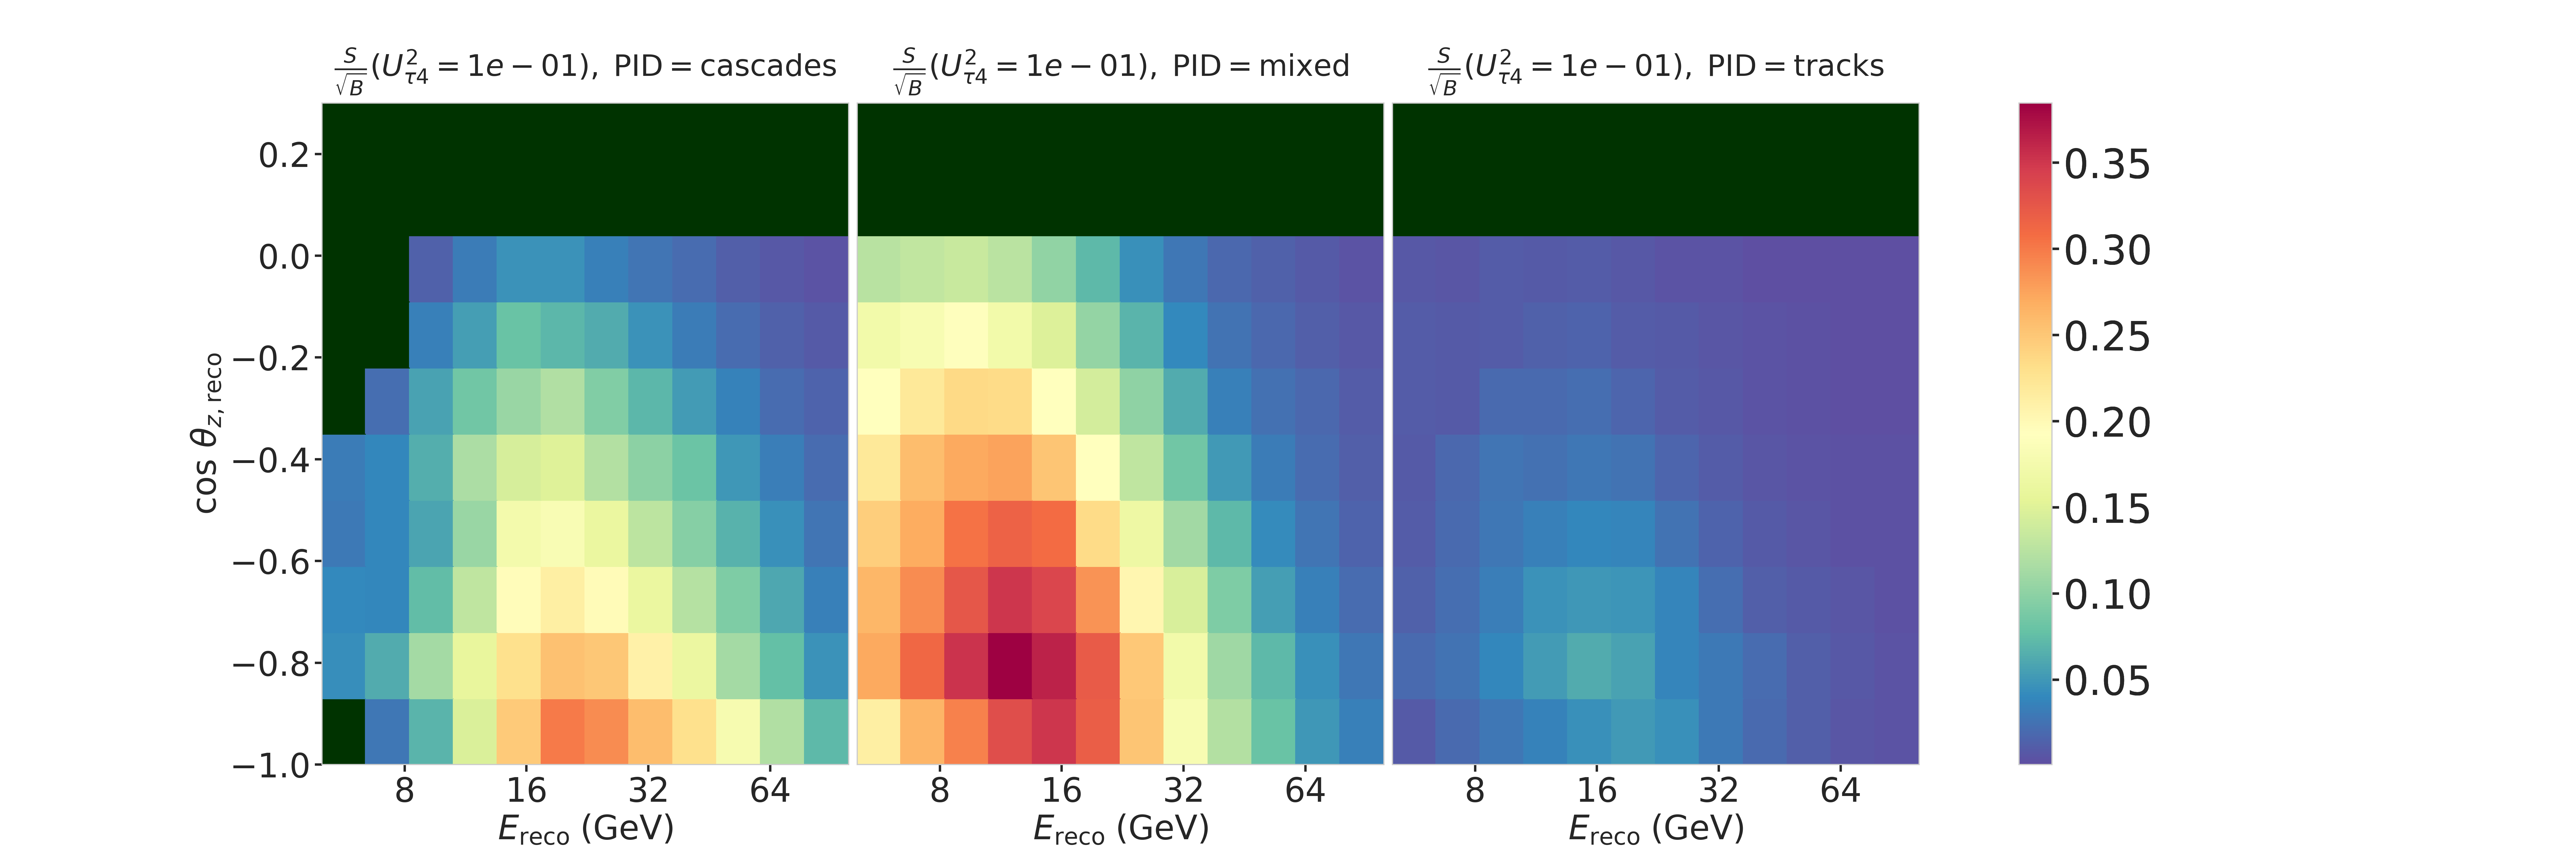
\includegraphics[trim=7cm 0cm 12cm 1cm, clip]{figures/results/labeled_s_to_sqrt_b_1.0_GeV_combined_U_tau4_sq_0.1000_total.png}
    \caption[]{}
    \labfig{s_to_sqrt_b_1.0_GeV_0.1_mixing}
\end{figure*}
\todo{fix caption (RED)}
\todo{remake without the top row of masked bins? add label to cbar and remove from title (RED)}


\section{Statistical Analysis} \labsec{analysis_principle}

\subsection{Test Statistic}

The measurements are performed by comparing the weighted MC to the data. Through variation of the nuisance and physics parameters that govern the weights, the best matching set of parameters can be found. The comparison is done using a modified $\chi^2$, defined as
\begin{equation}
    \chi^2_{\mathrm{mod}} = 
    \sum_{i \in \mathrm{bins}}^{}\frac{(N^{\rm{exp}}_i - N^{\mathrm{obs}}_i)^2}
    {N^{\rm{exp}}_i + (\sigma^{\mathrm{\nu}}_i)^2 + (\sigma^{\mathrm{\mu}}_i)^2 + (\sigma^{\mathrm{HNL}}_i)^2}
     + \sum_{j \in \mathrm{syst}}^{}\frac{(s_j - \hat{s_j})^2}{\sigma^2_{s_j}}
    \;,
    \labeq{mod-chi2-hnl}
\end{equation}
as the fit metric. It is designed such that taking the difference between a free fit and a fit with fixed parameters based on a chosen hypothesis, $\Delta\chi^2_{\mathrm{mod}}$, can be used as a \textit{test statistic (TS)} for hypothesis testing. The total even expectation is $N^{\rm{exp}}_i = N^{\mathrm{\nu}}_i + N^{\mathrm{\mu}}_i + N^{\mathrm{HNL}}_i$, where $N^{\mathrm{\nu}}_i$, $N^{\mathrm{\mu}}_i$, and $N^{\mathrm{HNL}}_i$ are the expected number of events in bin $i$ from neutrinos, atmospheric muons, and HNLs, while $N^{\mathrm{obs}}_i$ is the observed number of events in the bin. The expected number of events from each particle type is calculated by summing the weights of all events in the bin $N^{\mathrm{type}}_i = \sum_i^\rm{type}\omega_i$, with the statistical uncertainty being $(\sigma^{\mathrm{type}}_i)^2 = \sum_i^\rm{type}\omega_i^2$. The additional term in \refeq{mod-chi2-hnl} is included to apply a penalty term for prior knowledge of the systematic uncertainties of the parameters where they are known. $s_j$ are the systematic parameters that are varied in the fit, while $\hat{s_j}$ are their nominal values and $\sigma_{s_j}$ are the known uncertainties.

\todo{Do I want/need to include the description of the KDE muon estimation? (YELLOW)}


\subsection{Physics Parameters} \labsec{analysis_parameters}

The variable physics parameter in this analysis is the mixing between the HNL and the SM $\tau$ sector, $|U_{\tau4}|^2$. It can be changed continuously in the range of [\SI{0.0}, \SI{1.0}] by applying the weighting scheme described in \refsec{hnl_weighting_scheme}. The fit is initialized at an off-nominal value of 0.1. The other physics parameter, the mass $m_4$ of the HNL, is fixed to one of the three discrete masses to be tested, by using the corresponding sample of the HNL simulation described in \refsec{model_specific_simulation}.


\subsection{Nuisance Parameters} \labsec{analysis_systematics}

\todo{SB:
generally you are missing a lot of references, and I don't think its very nice to read all these ranges and so on in the text. Surely you can just have a table with the systematics you include, their allowed range and prior if applicable? You can choose whether or not you want to discuss some parameters in more detail here, but it should be a discussion of the physics and impact on the analysis. e.g. you can include some plots showing how a change in some of the nuisance parameters changes the event counts in the analysis binning (RED)
}


\begin{marginfigure}
    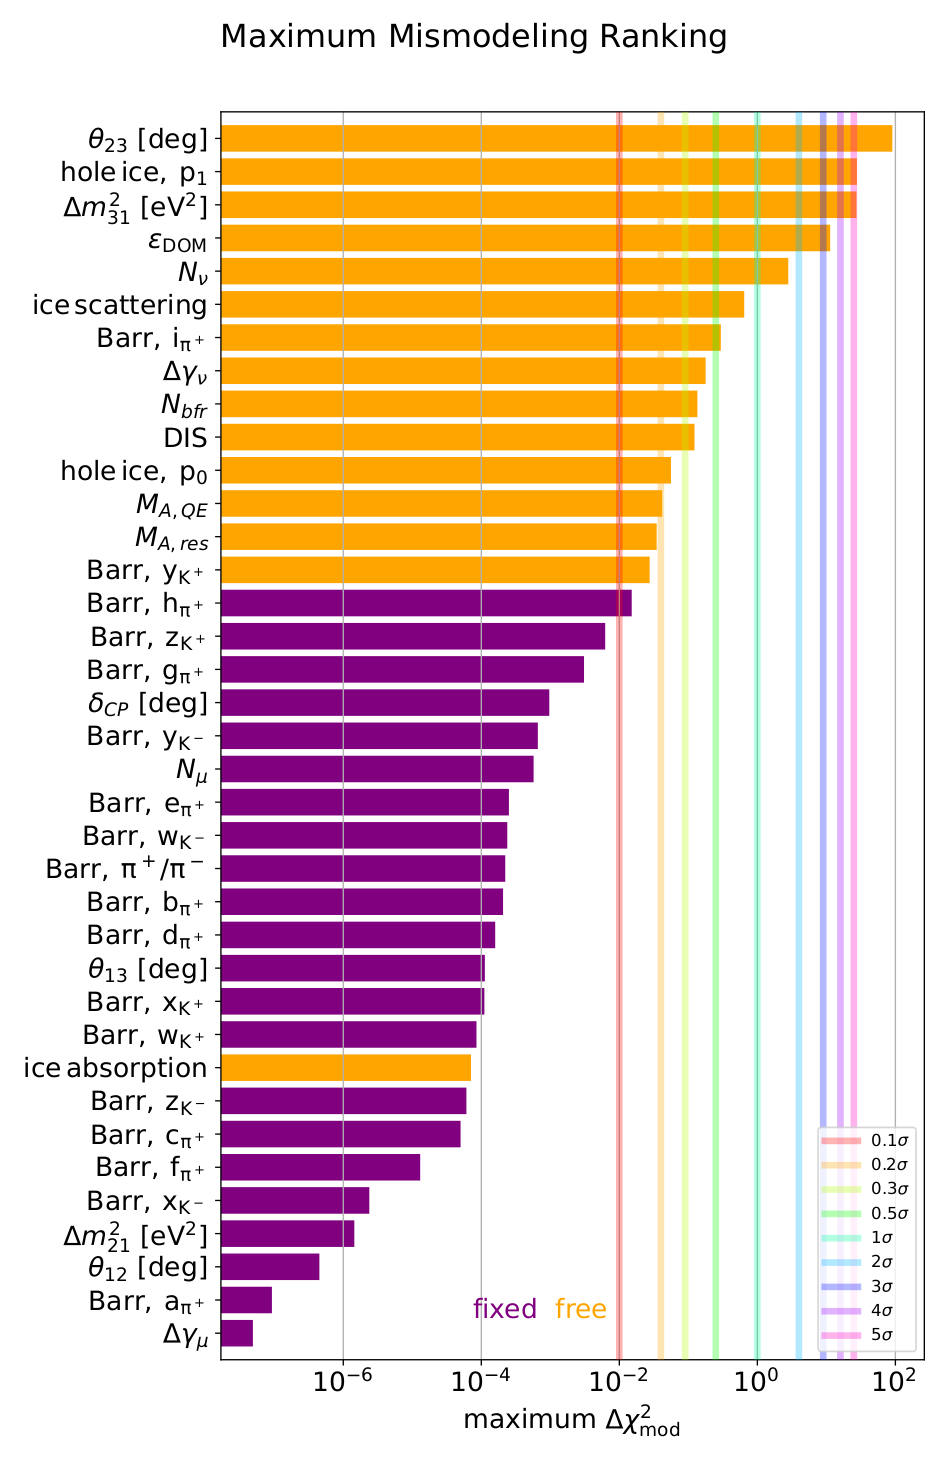
\includegraphics{figures/results/checks/plot_systematic_impact_ranking.png}
	\caption[xx]{"calculated at a mixing of 0.1 and for the 1.0 GeV sample"}
    \labfig{systematic_impact_test}
\end{marginfigure}
\todo{Blow up labels/legend/title and make it more readable in the margin or move it into the main text? (RED)}

To decide which systematic uncertainties should be included in the fit, we test the potential impact they have on the TS if they are neglected. The test is performed by creating Asimov data using the BG simulation and the HNL simulation of the \SI{1.0}{\gev} mass sample at a mixing value of $0.1$, which is chosen as a benchmark physics parameter and does not have a significant impact on the test. The systematic parameter of interest is set to a value above its nominal expectation, either pulled up by $+1\sigma$ or by an educated estimate for parameters without a well-defined uncertainty. A fit is performed fixing the systematic parameter of interest and leaving all additional parameters free. The resulting TS is the mis-modeling significance between this fit and a fit with all parameters free, which would result in a TS of 0.0 for this Asimov test. Parameters below a significance of \SI{0.1}{\sigma} are fixed, and the test is performed in an iterative manner until the final set of free parameters is found.

\reffig{systematic_impact_test} shows the resulting significances of one of these tests. The parameters tested are the systematic parameters introduced in \refsec{systematic_uncertainties} and the atmospheric oscillation parameters mentioned in \refsec{analysis_samples}. In the final selection of free parameters the Barr $h_{\pi^+}$ parameter was also left free\todo{elaborate why this is also done to cover the whole energy range for the Pion production, referencing the Barr Block plot that I haven't included yet :D (RED)} and the ice absorption is still kept free, despite showing a small significance. This is done because the bulk ice parameters are not well constrained and are known to have a large impact, which might be concealed in the test, due to correlations with the other parameters. In this test, the effect of correlations is challenging to consider, because only the impact of one parameter is tested at a time, using the overall mis-modeling significance as a measure. The mis-modeling could be reduced by a correlated parameter capturing the effect of the parameter of interest. For this reason a very conservative threshold of \SI{0.1}{\sigma} is chosen and some parameters below the threshold are still left free in the fit.

All nuisance parameters that are left free in the fit are summarized in \reftab{free_parameters}, showing their nominal values, the allowed fit ranges, and their Gaussian prior, if applicable. The scaling parameter $N_{\nu}$ is included to account for the overall normalization of the neutrino rate, and it has the identical effect on the SM neutrino events and the BSM HNL events, because they both originate from the same neutrino flux. Despite being known to $\sim$\SI{5}{\percent}\todo{Need cite here! (RED)} in this energy range, there is no prior applied to this parameter, because the fit itself is able to constrain it well, which can be seen by the large impact it shows in \reffig{systematic_impact_test}. Concerning the atmospheric neutrino flux, the CR power law flux correction factor $\Delta \gamma_\nu$ introduced in \refsec{flux_uncertainties} is included with nominal value of 0.0 which corresponds to a CR power law of $E^{-2}$. A slightly conservative prior of 0.1 is applied to the parameter, while latest measurements show an uncertainty of 0.05 \sidecite{PhysRevD.95.023012}.

% Additionally, the Barr $h_{\pi^+}$, Barr $i_{\pi^+}$, and Barr $y_{K^+}$ parameters of the Pion and Kaon production uncertainties are included with nominal values of $0.0$ and ranges of [$-0.75$, $0.75$], [$-3.05$, $3.05$], and [$-1.5$, $1.5$], respectively.\todo{say something about their priors (RED)}

% From the cross-section uncertainties introduced in \refsec{cross_section_uncertainties}, all three parameters, $\rm{DIS}$, $M_\rm{A,QE}$, and $M_\rm{A,res}$ are included in the fit with nominal values of $0.0$ for all of them and range [$-0.5$, $1.5$] for $\rm{DIS}$ and [$-2.0$, $2.0$] for the axial mass parameters $M_\rm{A,QE}$, and $M_\rm{A,res}$.\todo{say something about their priors (RED)}

All the detector systematic uncertainties are included in the fit. The DOM efficiency $\epsilon_{\rm{DOM}}$ is constrained by a Gaussian prior with a width of $0.1$, which is a conservative estimate based on the studies of the optical efficiency using minimum ionizing muons from \sidecite{JFeintzeig_phd, domeff_nick}.

% The hole ice model parameters $p_0$ and $p_1$ are included with nominal values of $0.101569$ and $-0.049344$, respectively, and ranges of [$-0.6$, $0.5$] and [$-0.2$, $0.2$]. The bulk ice absorption and scattering parameters are included with nominal values of $1.0$ and $1.05$, respectively, and ranges of [$0.85$, $1.15$] and [$0.9$, $1.2$]. They are unconstrained in the fit and the ranges are set to be conservative determined from calibration data\todo{cite?! (ORANGE)}

The two atmospheric neutrino oscillation parameters $\theta_{23}$ and $\Delta m^{2}_{31}$ are also included in the fit with nominal values of \SI{47.5047}{\degree} and \SI{2.475e-3}{\electronvolt^2}, respectively. Since they govern the shape and the strength of the tau neutrino flux, by defining the oscillation from $\nu_\mu$ to $\nu_\tau$, they are also relevant for the HNL signal shape.
% Their ranges are set to [\SI{0.0}{\degree}, \SI{90.0}{\degree}] and [\SI{0.001}{\electronvolt^2}, \SI{0.004}{\electronvolt^2}].

\todo{I should add some final level effects of some systematics on the 3D binning and maybe discuss how they are different from the signal shape, or so? (ORANGE)}

\begin{table}
    \begin{tabular}{ llll }
    \hline\hline
    \textbf{Parameter} & \textbf{Nominal} & \textbf{Range} & \textbf{Prior} \\
    \hline\hline
    $\theta_{23} [\si{\degree}]$ & 47.5047  & [0.0, 90.0] & - \\
    $\Delta m^{2}_{31} [\si{\electronvolt^2}]$ & 0.002475 & [0.001, 0.004] & - \\
    \hline
    $N_{\nu}$ & 1.0 & [0.1, 2.0] & - \\
    $\Delta \gamma_\nu$ & 0.0 & [-0.5, 0.5] & 0.1 \\
    $\rm{Barr} \, h_{\pi^+}$ & 0.0 & [-0.75, 0.75] & 0.15 \\
    $\rm{Barr} \, i_{\pi^+}$ & 0.0 & [-3.05, 3.05] & 0.61 \\
    $\rm{Barr} \, y_{K^+}$ & 0.0 & [-1.5, 1.5] & 0.3 \\
    \hline
    $\rm{DIS}$ & 0.0 & [-0.5, 1.5] & 1.0 \\
    $M_\rm{A,QE}$ & 0.0 & [-2.0, 2.0] & 1.0 \\
    $M_\rm{A,res}$ & 0.0 & [-2.0, 2.0] & 1.0\\
    \hline
    % $|U_{\tau 4}|^2$ & 0.0 & [0.0, 1.0] & - \\
    $\epsilon_{\rm{DOM}}$ & 1.0 & [0.8, 1.2] & 0.1 \\
    $\rm{hole \, ice} \, p_0$ & 0.101569 & [-0.6, 0.5] & - \\
    $\rm{hole \, ice} \, p_1$ & -0.049344  & [-0.2, 0.2] & - \\
    $\rm{bulk \, ice \, absorption}$ & 1.0 & [0.85, 1.15] & - \\
    $\rm{bulk \, ice \, scattering}$ & 1.05 & [0.9, 1.2] & - \\
    $N_\rm{bfr}$ & 0.0 & [-0.2, 1.2] & - \\
    \hline
    \end{tabular}
\caption[Nuisance parameter nominal values and fit ranges]{Systematic uncertainty parameters that are left free to float in the fit. Their allowed fit ranges are shown with the nominal value and the Gaussian prior width if applicable.}
\labtab{free_parameters}
\end{table}

\subsection{Treatment of Detector Response Uncertainties via a Likelihood-Free Inference Method} \labsec{ultrasurfaces}

\todo{I still need to write this section... (RED)}

\sidecite{Fischer_2023}

% Copy paste from OVS PRD about hypersurfaces (and interpolation of those):

% To evaluate the expected impact of detection uncertainties, data sets are produced with different variations of detector response, processed to the final level of selection, and then they are parameterized following a model of the uncertainties to evaluate how the final sample would look like for any reasonable choice of parameters. The parametrizations are done at the analysis bin level, assuming that every effect considered is independent and that they can be approximated by a linear function. Under these assumptions we can compute a reweighting factor in every bin that depends on $N$ parameters, which correspond to the number of systematic effects being considered, plus an offset $c$, as

% \begin{equation}
%     f(p_1,...,p_N)=c+\sum_{n=1}^N m_n \Delta p_n.
% \end{equation}
% Here $m_n$ are the reweighting factors obtained from simulation sets with a systematic variation and $\Delta p_n$ is the test value of a specific systematic variation.

% The fit of the parameters $m_n$ is done over all systematic MC sets, reducing the uncertainty on the MC prediction in each bin as a side effect since the error on the fitted function is smaller than the statistical error from the nominal MC set. The set of all fitted functions in all histogram bins are called ``hypersurfaces". An example of such a fit from a single bin, projected onto one dimension, is shown in Fig. \ref{fig:hypersurface-example}. %The result of using hypersurfaces accurately predicted the bin content of simulation sets that were left out of the parameterization.

% The event counts coming from different flavors and interactions have a different response to varying the same detector parameter. Therefore, the hypersurfaces in each bin are fit separately for three groups of events:
% \begin{itemize}
%     \item ($\nu_{\mathrm{all}} + \bar{\nu}_{\mathrm{all}}$) NC + ($\nu_e + \bar{\nu}_e$) CC: These events all produce cascade signatures in the detector.
%     \item ($\nu_\tau + \bar{\nu}_\tau$) CC: These interactions may differ from the previous group because they have a production threshold of $E_\nu \gtrsim 3.5\,\mathrm{GeV}$ and also produce muons with a branching ratio of 17\%.
%     \item ($\nu_\mu + \bar{\nu}_\mu$) CC: These interactions produce track-like signatures.
% \end{itemize}

% % \begin{figure}[t!]
% %     \centering
% %     \includegraphics[width=.95\linewidth]{Figures/detector_syst/hypersurface_example_v5.pdf}
% %     \caption{Example of a hypersurface function in one bin projected on the DOM efficiency dimension. Each data point corresponds to one systematic set. Translucent datapoints are from sets where one or more systematic parameter \emph{besides} DOM efficiency is off-nominal. Those points are projected along the fitted plane to the nominal point. Several systematic sets have a nominal DOM efficiency of 1.0. The translucent error band corresponds to the standard deviation of the fitted function.}
% %     \label{fig:hypersurface-example}
% % \end{figure}

% The distribution of $\chi^{2}$/d.o.f. from the fits in all analysis bins is used as a diagnostic to ensure that the fitted, linear hypersurfaces provide a good estimate for the expected number of events for the full range of simulated detector configurations. We find that the means of these $\chi^{2}$/d.o.f. distributions are all consistent with 1.0 as expected from good fits for each of the three categories described above (NC + $\nu_{e}$ CC, $\nu_{\tau}$ CC and $\nu_{\mu}$ CC). Attempts to use higher order polynomial fits did not yield a significantly improved $\chi^{2}$/d.o.f., and in fact often rendered the fits less stable. 

% To produce the histograms for fitting the hypersurfaces, a choice must be made for the values of flux, cross-section and oscillation parameters. We found that the hypersurface fits are sensitive to the choice of parameters that have correlations with the effect they encode. Most notably, this effect is observed between the mass splitting and DOM optical efficiency as demonstrated in Fig.~\ref{fig:interpolatedHS}, which shows the difference between fitted hypersurface gradients for the DOM efficiency dimension for two values of $\Delta m^{2}_{32}$. 
% %Moreover, we found that assuming the wrong mass splitting can introduce a significant bias in the measurement if the fitted DOM efficiency is pulled by only 1$\sigma$. 

% This problem arises because we are only fitting the hypersurfaces in reconstructed phase space, without accounting for the different true energy and zenith distributions of MC in each analysis bin, which change with each detector systematic variation. To mitigate this problem, we fit the hypersurfaces for 20 different values in mass splitting between $1.5\times 10^{-3}\,\mathrm{eV}^2$ and $3.5\times 10^{-3}\,\mathrm{eV}^2$, and then apply a piece-wise linear interpolation to all slopes, intercepts and covariance matrix elements. The oscillation parameter fit can then dynamically adapt the hypersurfaces for each value of $\Delta m^{2}_{32}$ that is tested using these interpolated functions. The effects of other parameter choices were evaluated as well, but none were found to introduce a significant bias.


\subsection{Low Energy Analysis Framework} \labsec{analysis_framework}

The analysis is performed using the \textsc{PISA} \sidecite{pisa_paper} \cite{pisa_software} software framework, which was developed to perform analyses "of small signals in high-statistics neutrino oscillation experiments". It is used to generate the expected event distributions from several MC samples, which can then be compared to the observed data. The expectation for each sample is calculated in parallel, applying physics and nuisance parameter effects in a stage-wise manner, before combining the final expectation from all the samples.\todo{Do I want more information about the different pipelines and stages? Could link back to the extra stage I wrote and add the earth model and oscillation calculation information here, I guess?! (ORANGE)}


\section{Analysis Checks}

Fitting to data is performed in a \textit{blind} manner, where the analyzer does not immediately see the fitted physics and nuisance parameter values, but first checks that a set of pre-defined \textit{goodness of fit (GOF)} criteria are fulfilled.
% At this point changes to the analysis can still be made, if the criteria are not met.
This is done to circumvent the so-called \textit{confirmation bias} \sidecite{confirmation_bias}, where the analyzer might be tempted to construct the analysis in a way that confirms their expectation. After the GOF criteria are met to satisfaction, the fit results are unblinded and the full result can be revealed. Before these blind fits to data are performed, the robustness of the analysis method is tested using pseudo-data that is generated from the MC.


\subsection{Minimization Robustness} \labsec{asimov_inject_recover}

To find the set of parameters that best describes the data, a staged minimization routine is used. In the first stage, a fit with coarse minimizer settings is performed to find a rough estimate of the \textit{best fit point (BFP)}. In the second stage, the fit is performed again in both octants\sidenote{There is a degeneracy between the lower octant ($\theta_{23}<\SI{45}{\degree}$) and the upper octant ($\theta_{23}>\SI{45}{\degree}$), which can lead to fit metric minima (local and global) at two positions that are mirrored around \SI{45}{\degree} in $\theta_{23}$.} of $\theta_{23}$, starting from the BFP of the coarse fit. For each individual fit the \textit{MIGRAD} routine of \textsc{iminuit} \sidecite{iminuit_v2.17.0} is used to minimize the $\chi^2_{\mathrm{mod}}$ fit metric defined in \refeq{mod-chi2-hnl}. Iminuit is a fast, python compatible minimizer based on the \textsc{Minuit2} C++ library \sidecite{og_minuit}. The individual minimizer settings for both stages are shown in \reftab{minimization_settings}.

\begin{margintable}
    \small
        \begin{tabular}{ llll }
        \hline\hline
        \textbf{Fit} & \textbf{Err.} & \textbf{Prec.} & \textbf{Tol.} \\
        \hline\hline
        Coarse & 1e-1 & 1e-8 & 1e-1 \\
        Fine & 1e-5 & 1e-14 & 1e-5 \\
        \hline
        \end{tabular}
    \caption[Staged minimization routine settings]{Migrad settings for the two stages in the minimization routine. \textit{Err.} are the step size for the numerical gradient estimation, \textit{Prec.} is the precision with which the LLH is calculated, and \textit{Tol.} is the tolerance for the minimization.}
    \labtab{minimization_settings}
\end{margintable}

To test the minimization routine and to make sure it consistently recovers any physics parameters, pseudo-data sets are produced from the MC by choosing the nominal nuisance parameters and specific physics parameters, without adding any statistical or systematic fluctuations to it. These so-called \textit{Asimov}\sidenote{A pseudo-data set without statistical fluctuations is called Asimov data set.} data sets are then fit back with the full analysis chain. This type of test is called \textit{Asimov inject/recover test}. A set of mixing values between $10^{-3}$ and $10^{0}$ is injected and fit back.
% Even though this range is well within the excluded regions by other experiments, discussed in \refsec{HNL_mixing_constraints}, this covers the current sensitive region of the analysis in IceCube DeepCore.
Without fluctuations the fit is expected to always recover the injected parameters (both physics and nuisance parameters). The fitted mixing values from the Asimov inject/recover tests are compared to the true injected values in \reffig{asimov_inject_recover_0.6_GeV} for the \SI{0.6}{\gev} sample. As expected, the fit is always able to recover the injected physics parameter and the nuisance parameters.

\todo{Put all three mass samples in one plot and adjust the text to it? Remove "fit start" from legend. (RED)}
\todo{Mention that the mis-modeling (what it is) is at the order of 1e-07 for all of them (check again) and refer to the deviations in the mixing to be not relevant because of that! (RED)}

% The same is true for the other mass samples and the additional plots for the other mass samples can be found in \refsec{asimov_inject_recover_appendix}.

\begin{figure}[h]
    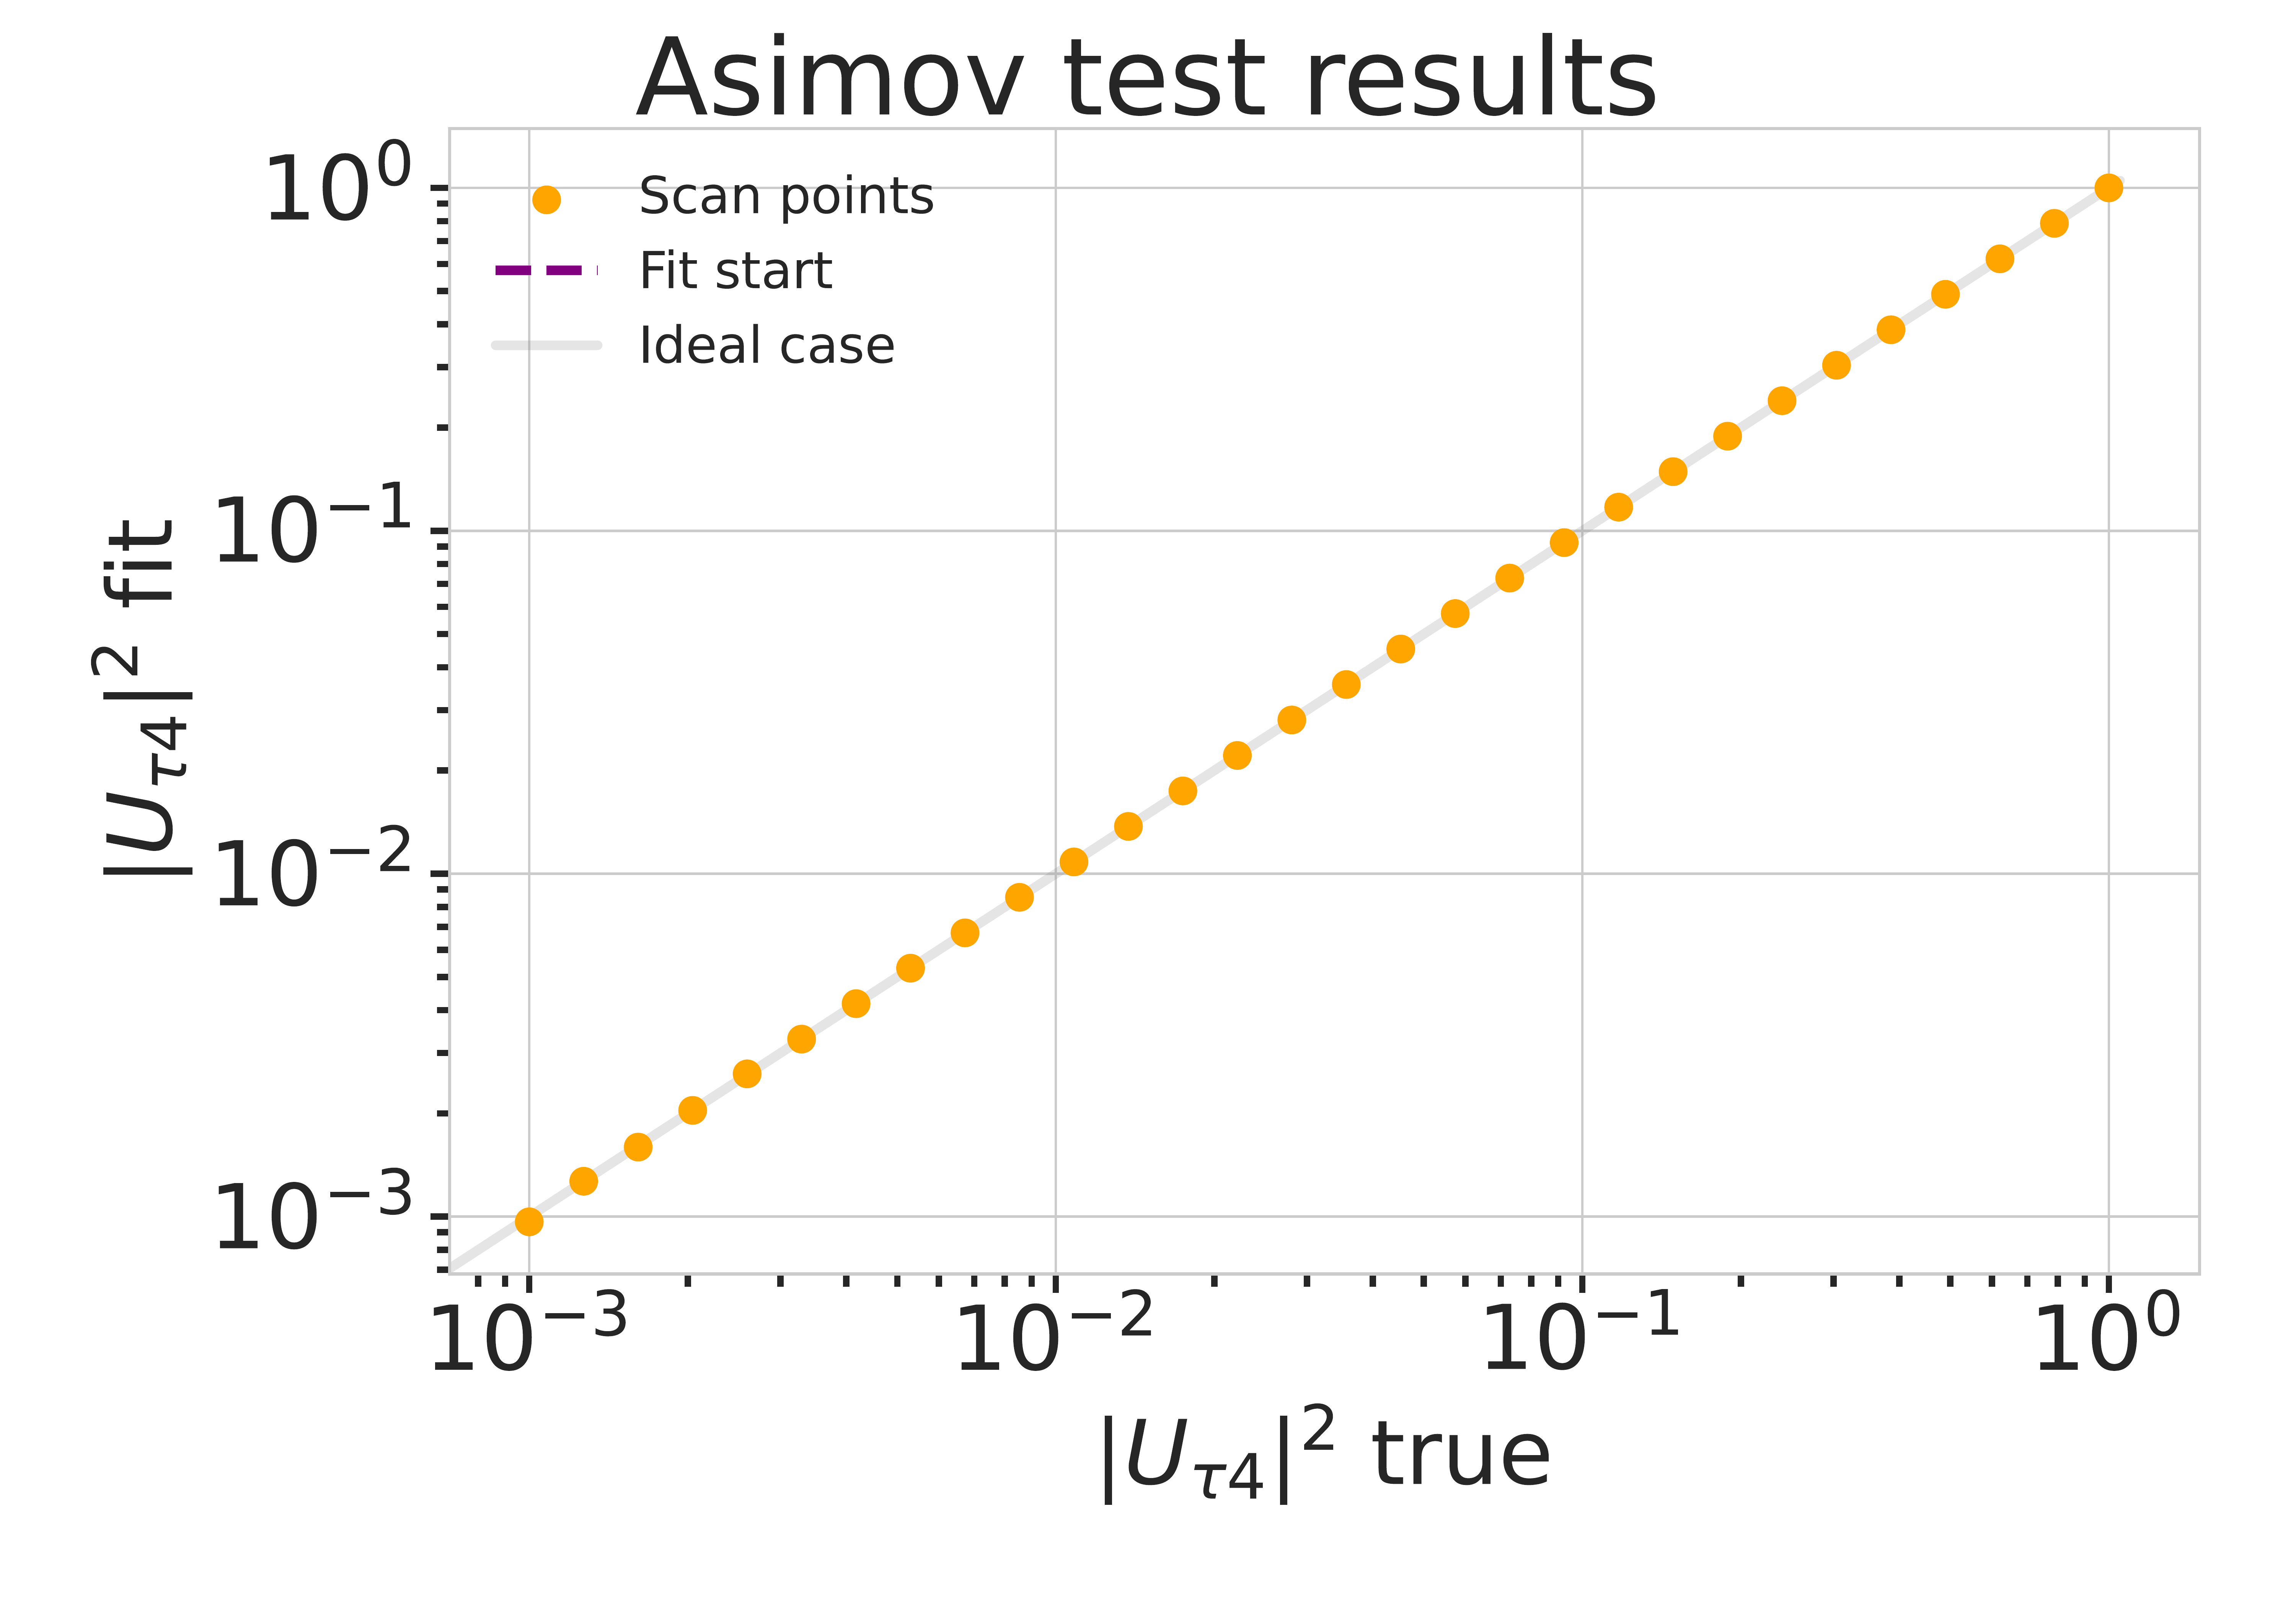
\includegraphics{figures/results/checks/asimov_scan_0.6_GeV-01.png}
	\caption[Asimov inject/recover test (\SI{0.6}{\gev})]{Asimov inject/recover test for the \SI{0.6}{\gev} mass sample. Mixing values between $10^{-3}$ and $10^{0}$ are injected and fit back with the full analysis chain. The injected parameter is always recovered within the statistical uncertainty.}
    \labfig{asimov_inject_recover_0.6_GeV}
\end{figure}


\subsection{Goodness of Fit} \labsec{pseudo_data_ensemble}

To estimate the GOF, pseudo-data is generated from the MC by injecting the BFP parameters as true parameters and then fluctuating the expected bin counts to account for MC uncertainty and Poisson fluctuations in data. First, the expectation value of each bin is drawn from a Gaussian distribution centered at the nominal expectation value with a standard deviation corresponding to the MC uncertainty of the bin. Based on this sampled expectation value, each bin count is drawn from a Poisson distribution, independently, to get the final pseudo-data set. These pseudo-data sets are then fit back with the analysis chain. By comparing the distribution of fit metric values from this \textit{ensemble} of pseudo-data trials to the fit metric of the fit to real data, a p-value can be calculated. The p-value is the probability of finding a value at least as large as the one from the data fit. \reffig{pseudo_data_ensembles}\todo{Add 3D BFP-data pull distribution for one mass (they look the same, no?) (RED)} shows the distribution from the ensemble tests for the \SI{0.6}{\gev} mass sample and the observed value from the fit, resulting in a p-value of \SI{28.5}{\percent}. The p-values for the \SI{0.3}{\gev} and \SI{1.0}{\gev} are \SI{28.3}{\percent} and \SI{26.0}{\percent}, respectively, and the corresponding plots are shown in \refsec{pseudo_data_ensemble_appendix}. Based on this test, it is concluded that the fit result is compatible with the expectation from the ensemble of pseudo-data trials.

\begin{figure*}[h]
    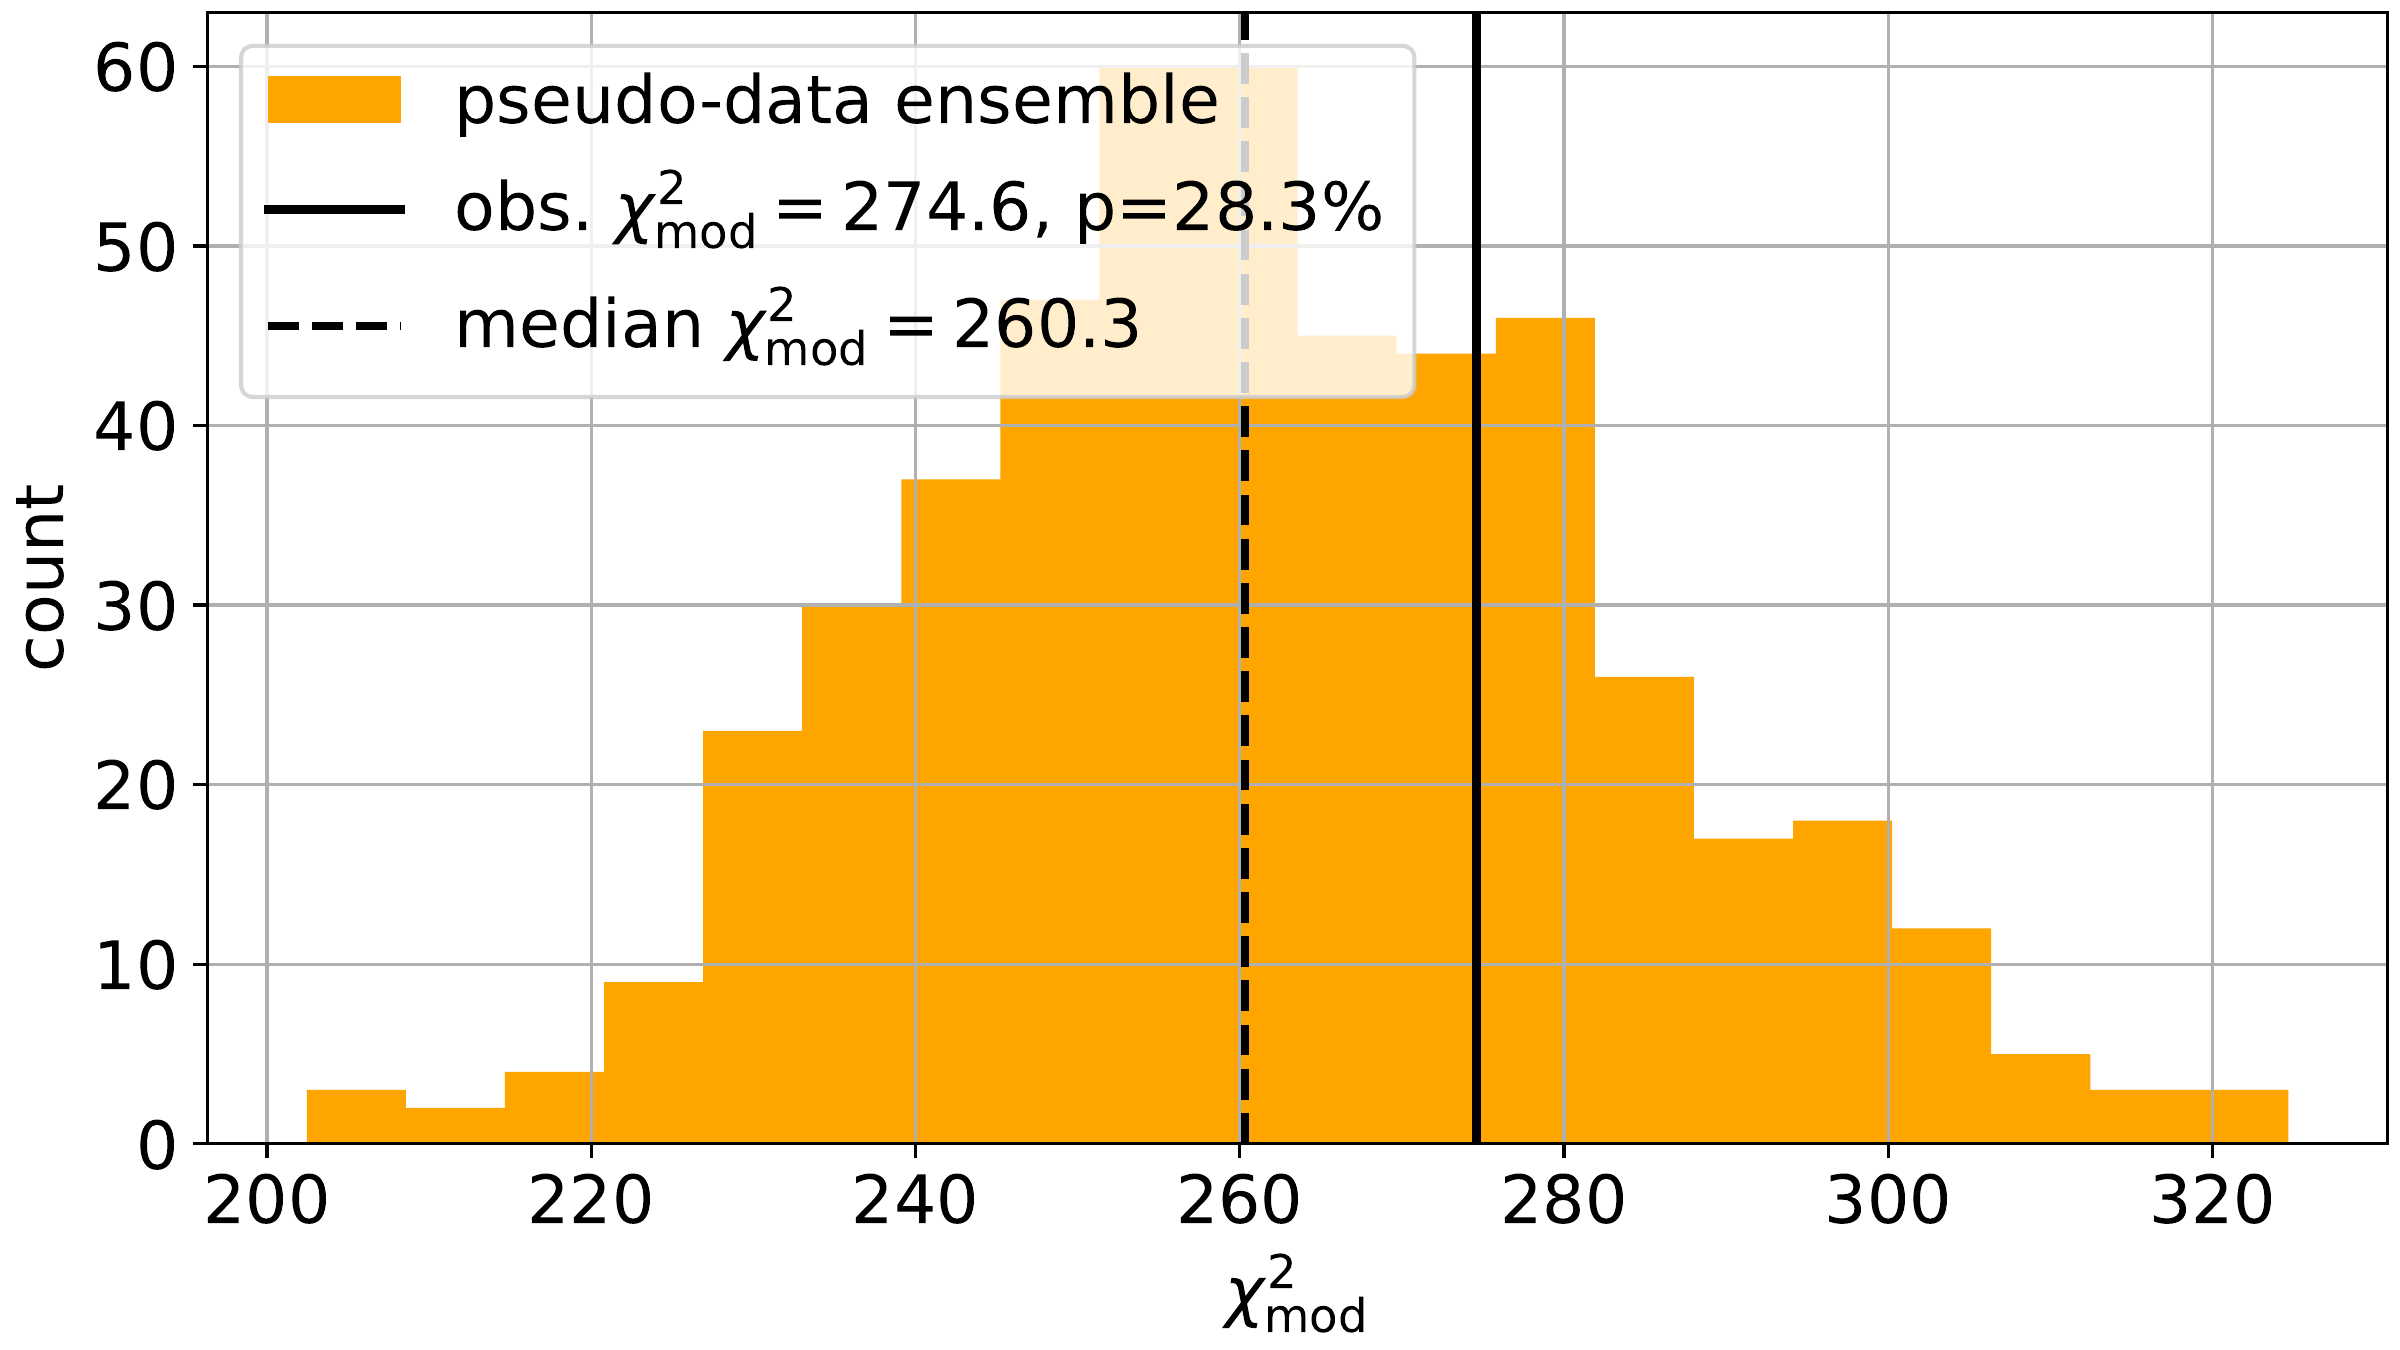
\includegraphics[width=0.32\linewidth]{figures/results/blind_fits/full_blind_fit_0.3_GeV_gauss_plus_poisson_step_3_4-1.png}
    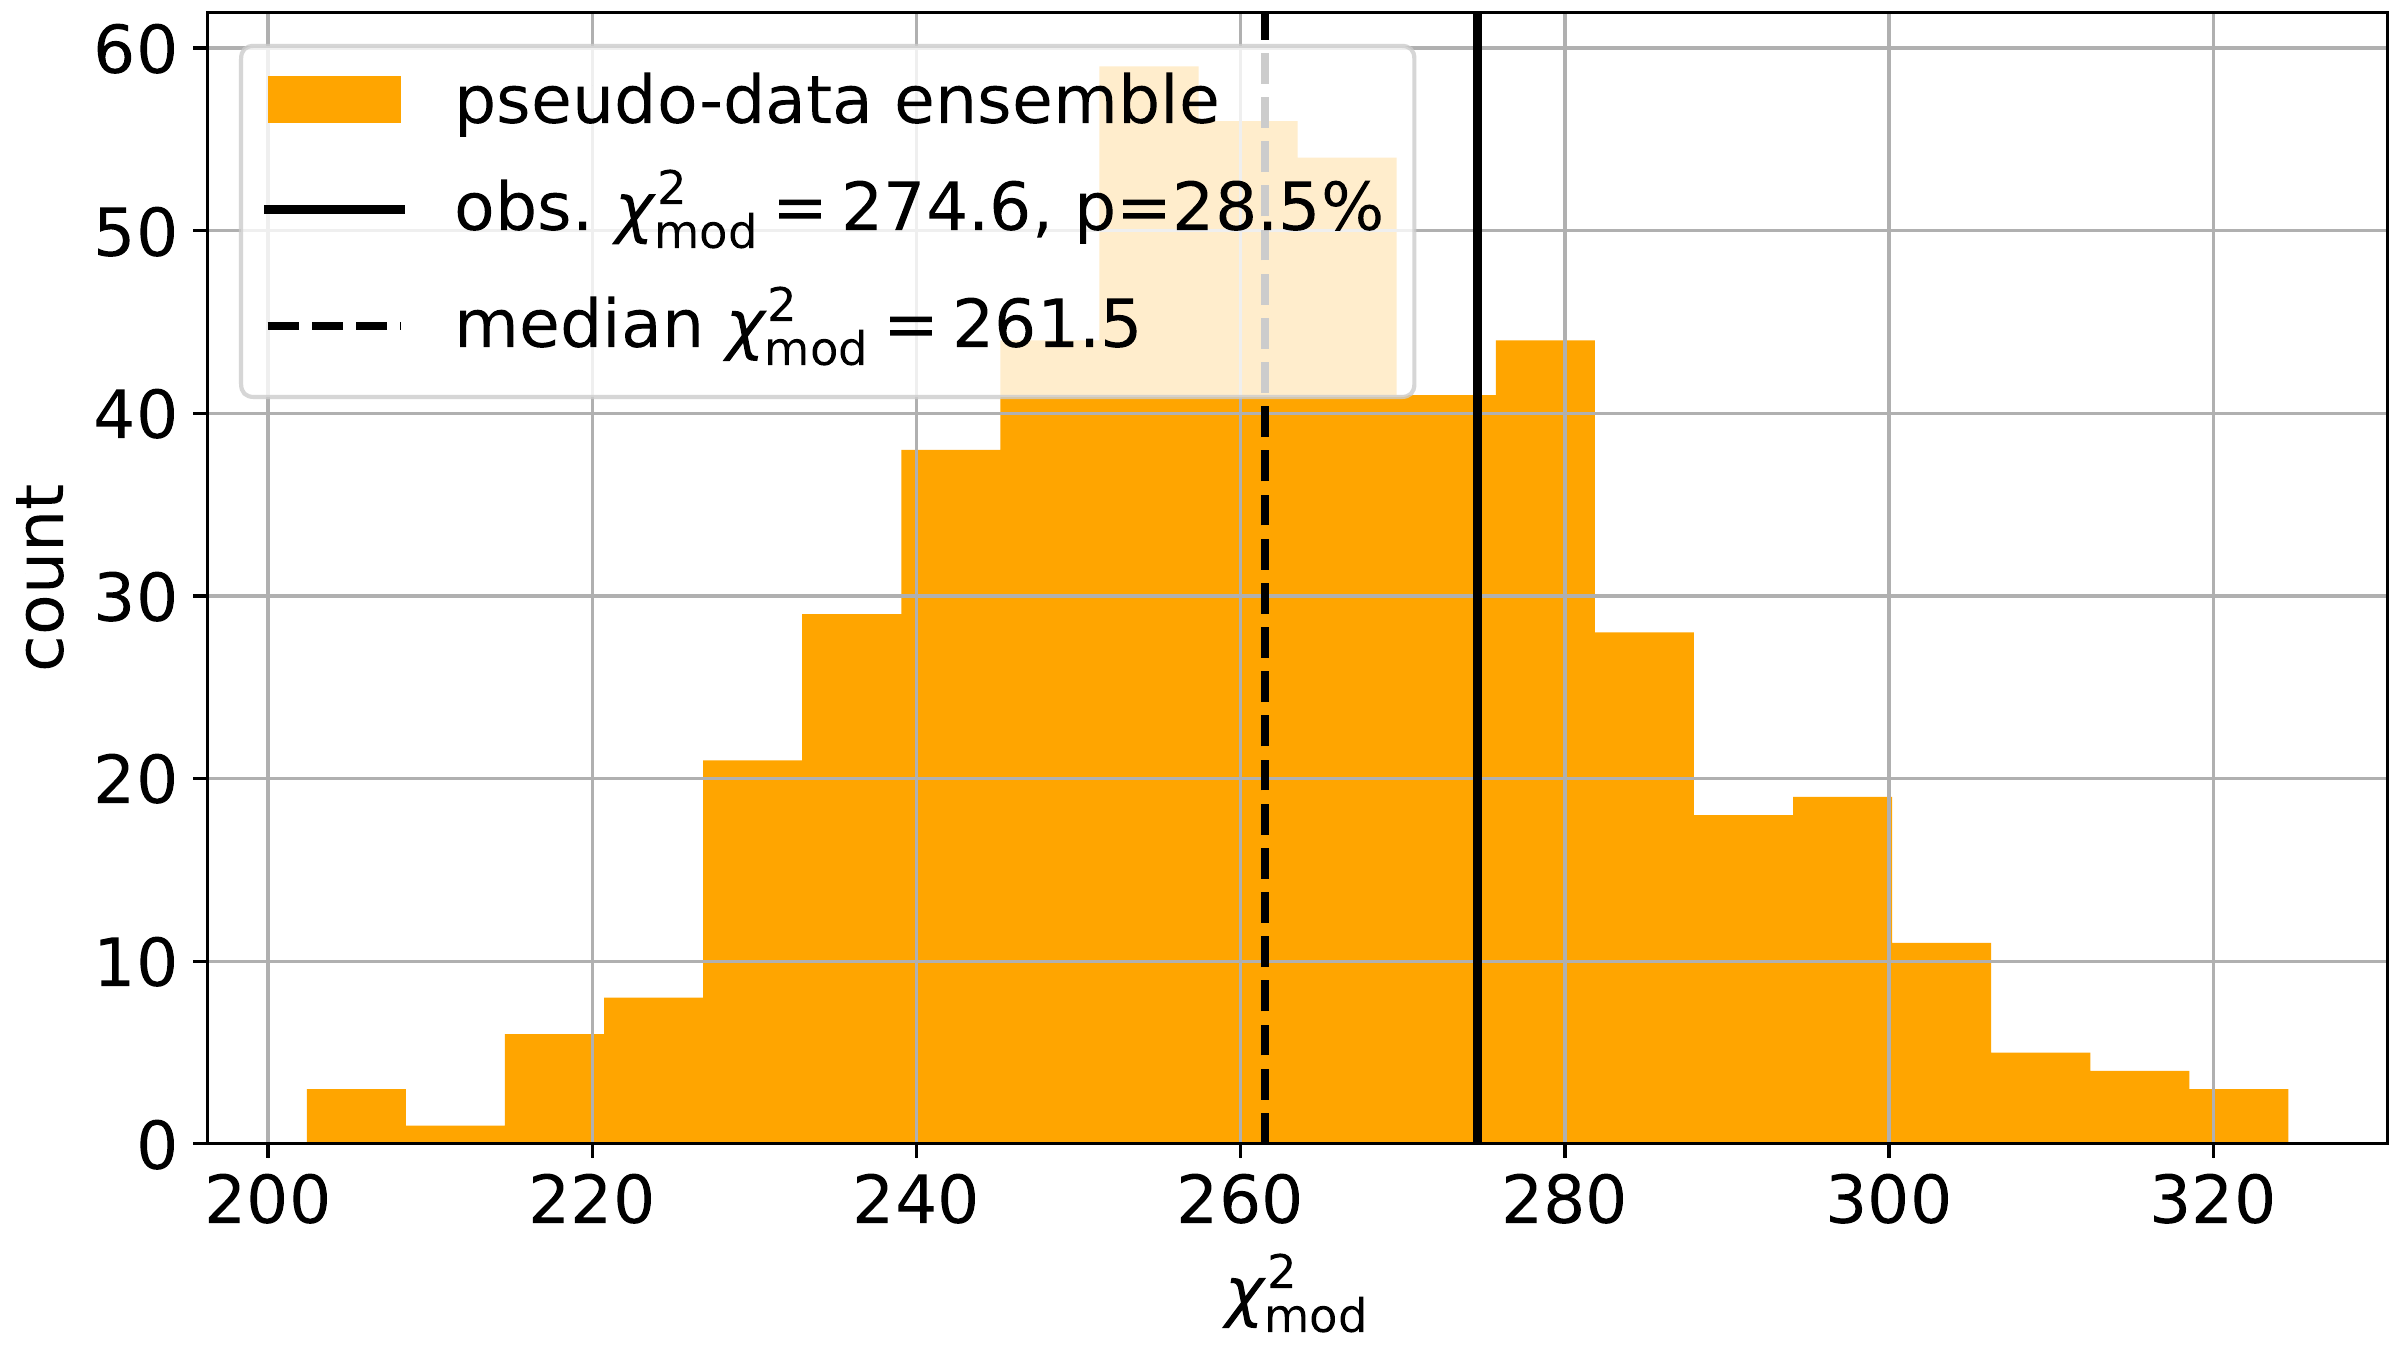
\includegraphics[width=0.32\linewidth]{figures/results/blind_fits/full_blind_fit_0.6_GeV_gauss_plus_poisson_step_3_4-1.png}
    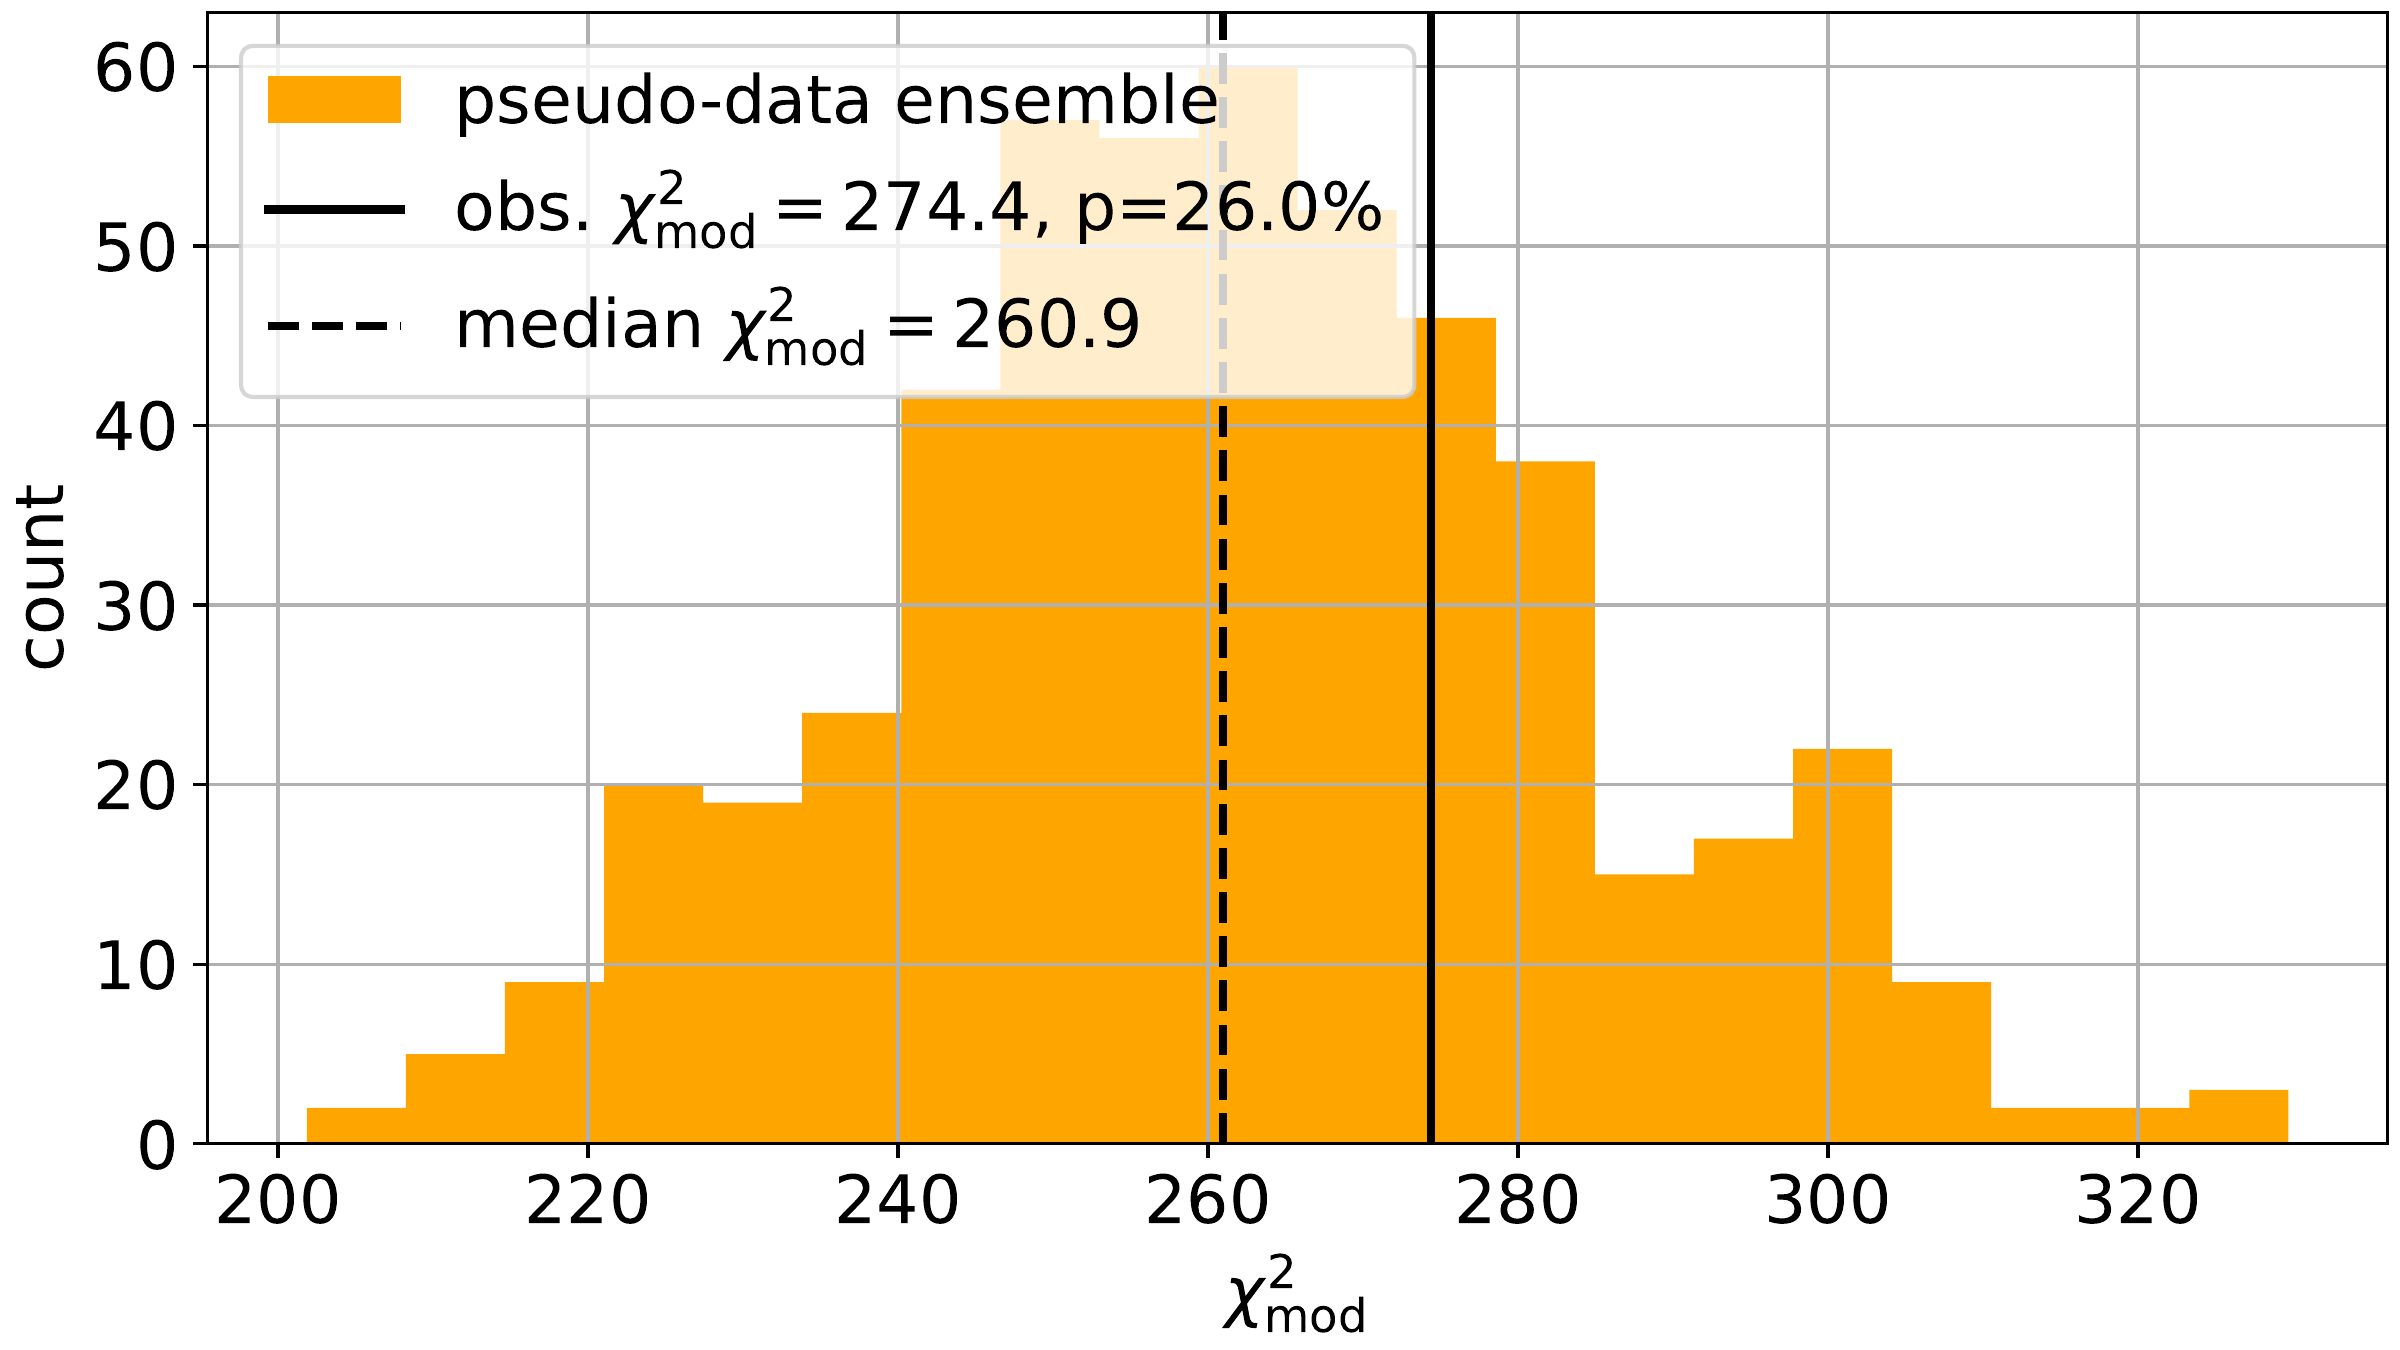
\includegraphics[width=0.32\linewidth]{figures/results/blind_fits/full_blind_fit_1.0_GeV_gauss_plus_poisson_step_3_4-1.png}
	\caption[Pseudo-data trials fit metric distribution (\SI{0.6}{\gev})]{Observed fit metric and fit metric distribution from pseudo-data trials for the \SI{0.6}{\gev} mass sample.}
    \labfig{pseudo_data_ensembles}
\end{figure*}
\todo{fix dimension to fit them in one row! (RED)}


\subsection{Data/MC Agreement}

At the BFP, the agreement between the data and simulation is probed by comparing the 1-dimensional analysis distributions for PID, energy, and cosine of the zenith angle. As an example, two distributions\todo{specify which they are, once I have them (RED)} for the \SI{0.6}{\gev} mass sample are shown in \reffig{data_mc_agreement_0.6_GeV}. The data is compared to the total MC expectation, which is also split up into its composing parts. Good agreement can be observed in the pull distributions and is quantified by a reduced $\chi^2$, which is close to \SI{1.0} for all distributions. The reduced $\chi^2$ for all investigated distributions is listed in \reftab{data_mc_agreement}, while the distributions themselves can be found in \refsec{data_mc_agreement_appendix}.

\todo{add 1-d data/mc agreement for example mass sample (0.6?) and all 3 analysis variables (RED)}
\todo{add table with reduced chi2 for all 1-d distributions (RED)}


\section{Results}

\subsection{Best Fit Nuisance Parameters}

The resulting nuisance parameter values from the fits are illustrated in \reffig{best_fit_deltas_normed}, where the differences to the nominal values are shown, normalized by the distance to the closest boundary. The results from all three fits are shown in the same plot and the fits prefer values of the same size for all three mass samples. For parameters that had a Gaussian prior, the \SI{1}{\sigma} range is also displayed. As was already confirmed during the blind fit procedure, all fitted parameters are within this range.
% , but the $\rm{Barr} \; h_{\pi^+}$ parameter is smaller and the $\rm{Barr} \; i_{\pi^+}$ is larger than expected, both being very close within the $+$\SI{1}{\sigma} and the $-$\SI{1}{\sigma} range, respectively. The $\rm{DIS}$ parameter fits to a smaller value than the nominal and all ice parameters, both $\rm{hole \, ice} \; p_0$, and $p_1$ as well as $\rm{bulk \, ice \, absorption}$, and $\rm{scattering}$ are found at values lower than the nominal.
The effective ice model parameter, $N_\rm{bfr}$, prefers a value of $\sim$\SI{0.74}, indicating that the data fits better to an ice model that includes real birefringence effects \todo{Cite (again)! (RED)} during photon propagation. For completeness's sake, the explicit results are listed in \reftab{best_fit_parameters}. There, the nominal values and the absolute differences to the best fit value are also presented.

\todo{Compare here the best fit oscillation parameters to the FLERCNN results and try to quantify it, stating the pitfalls of the comparitions (satistically fully dependent) (RED)}

\begin{figure*}[h]
    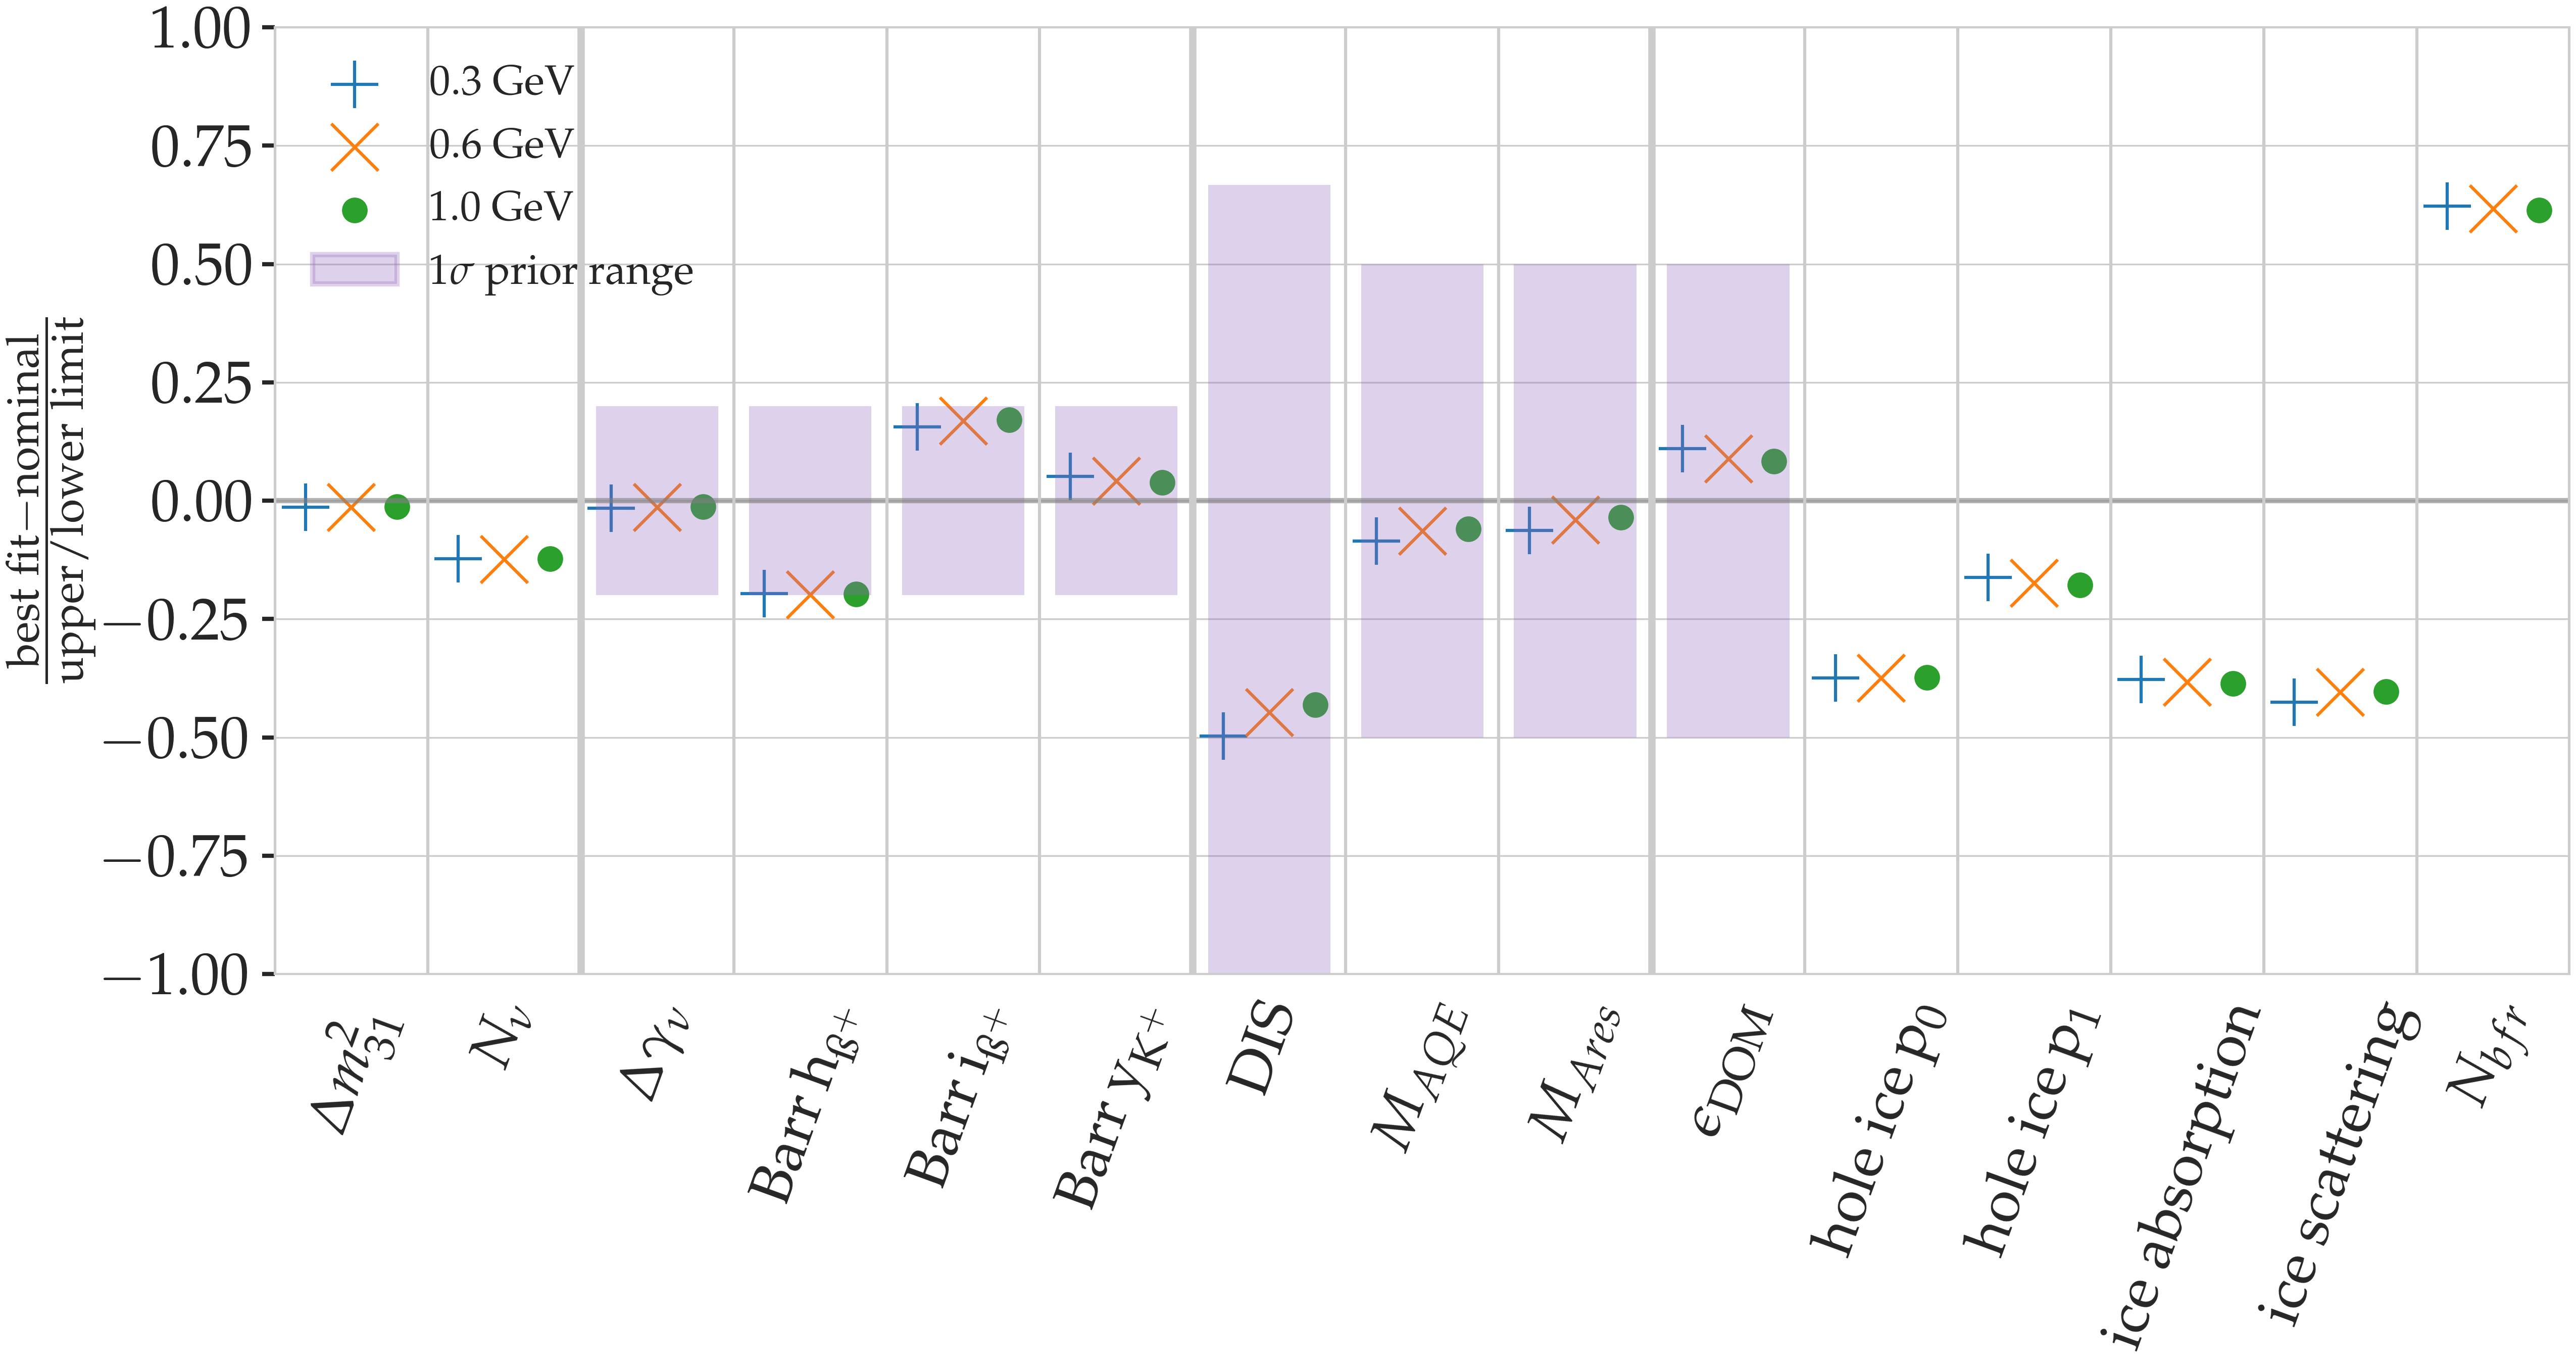
\includegraphics{figures/results/best_fit/hnl_analysis_best_fit_deltas_normed_dist_to_nominal_correct_0.6_fit_updated.png}
	\caption[Best fit nuisance parameter distances to nominal]{Best fit nuisance parameter distances to the nominal values, normalized by the distance to the closest boundary. For parameters with a Gaussian prior, the $+$\SI{1}{\sigma} range is also shown.}
    \labfig{best_fit_deltas_normed}
\end{figure*}

\todo{Show best fit hole ice angular acceptance compared to nominal and flasher/in-situ fits, maybe? (YELLOW)}
\todo{Discuss what it means that the parameters are at these values? Here, or somewhere else? (RED)}


\subsection{Best Fit Parameters and Limits}

The fitted mixing values are
\begin{align*}
    |U_{\tau4}|^2(\SI{0.3}{\gev}) &= 0.003^{+0.084} \;, \\
    |U_{\tau4}|^2(\SI{0.6}{\gev}) &= 0.080^{+0.134} \;, \rm{and} \\
    |U_{\tau4}|^2(\SI{1.0}{\gev}) &= 0.106^{+0.132} \;,
\end{align*}
with their $+$\SI{1}{\sigma} uncertainty. All of them are compatible with the null hypothesis of \SI{0.0} mixing, although the \SI{0.6}{\gev} and \SI{1.0}{\gev} fits indicate a mixing value of \SI{0.08} and \SI{0.106}, respectiveley. The best fit mixing values and the corresponding upper limits at \SI{68}{\percent} and \SI{90}{\percent} \textit{confidence level (CL)} are listed in \reftab{best_fit_parameters_and_confidence_levels}, also showing the $p$-value to reject the null hypothesis. The CLs and $p$-value are estimated by assuming that \textit{Wilks' theorem} \sidecite{the_not_to_be_mentioned_theorem} holds, meaning that the TS follows a $\chi^2$ distribution with one degree of freedom.

\begin{table}[h]
    % \footnotesize
    
    % \begin{tabular}{ lllll }
    \begin{tabular}{ ccccc }
        \hline\hline

        \textbf{HNL mass} & \textbf{$|U_{\tau4}|^2$} & \textbf{68 \si{\percent} CL} & \textbf{90 \si{\percent} CL} & \textbf{NH $p$-value} \\
    
        \hline\hline

        \SI{0.3}{\gev} & 0.003 & 0.087 & 0.194 & \SI{0.97}{} \\
        \SI{0.6}{\gev} & 0.080 & 0.214 & 0.355 & \SI{0.79}{} \\
        \SI{1.0}{\gev} & 0.106 & 0.238 & 0.396 & \SI{0.63}{} \\

        \hline
    \end{tabular}

    \caption[xx]{xx}
    \labtab{best_fit_parameters_and_confidence_levels}
\end{table}
\todo{fix table caption (RED)}

\reffig{brazil_bands} shows the observed TS profiles as a function of $|U_{\tau4}|^2$ for all three fits. The TS profile is the difference in $\chi^2_{\mathrm{mod}}$ between the free fit and a fit where the mixing is fixed to a specific value. Also shown is the expected TS profile, based on 100 pseudo-data trials, produced at the BFP and then fluctuated using both Poisson and Gaussian fluctuations, to include the data and the MC uncertainty as was explained in \refsec{pseudo_data_ensemble}. The median expectation and the \SI{68}{\percent} and \SI{90}{\percent} bands are shown and the observed TS profiles lie within the \SI{68}{\percent} band for all three, confirming that they are compatible with data fluctuations. For the \SI{0.3}{\gev} fit, the observed contour is slightly left of the median expectation, meaning that the observed upper limits in $|U_{\tau4}|^2$ are slightly stronger than expected. For the \SI{0.6}{\gev} the opposite is the case and the observed upper limit is therefore slightly weaker than expected. For the \SI{1.0}{\gev} fit, the observed upper limit is very close to the median expectation in the region where the \SI{68}{\percent} and \SI{90}{\percent} CLs thresholds are crossed\todo{add horizontal CL lines?}. The observed upper limits are also shown in \reftab{best_fit_parameters_and_confidence_levels}.

\begin{figure*}[h]
    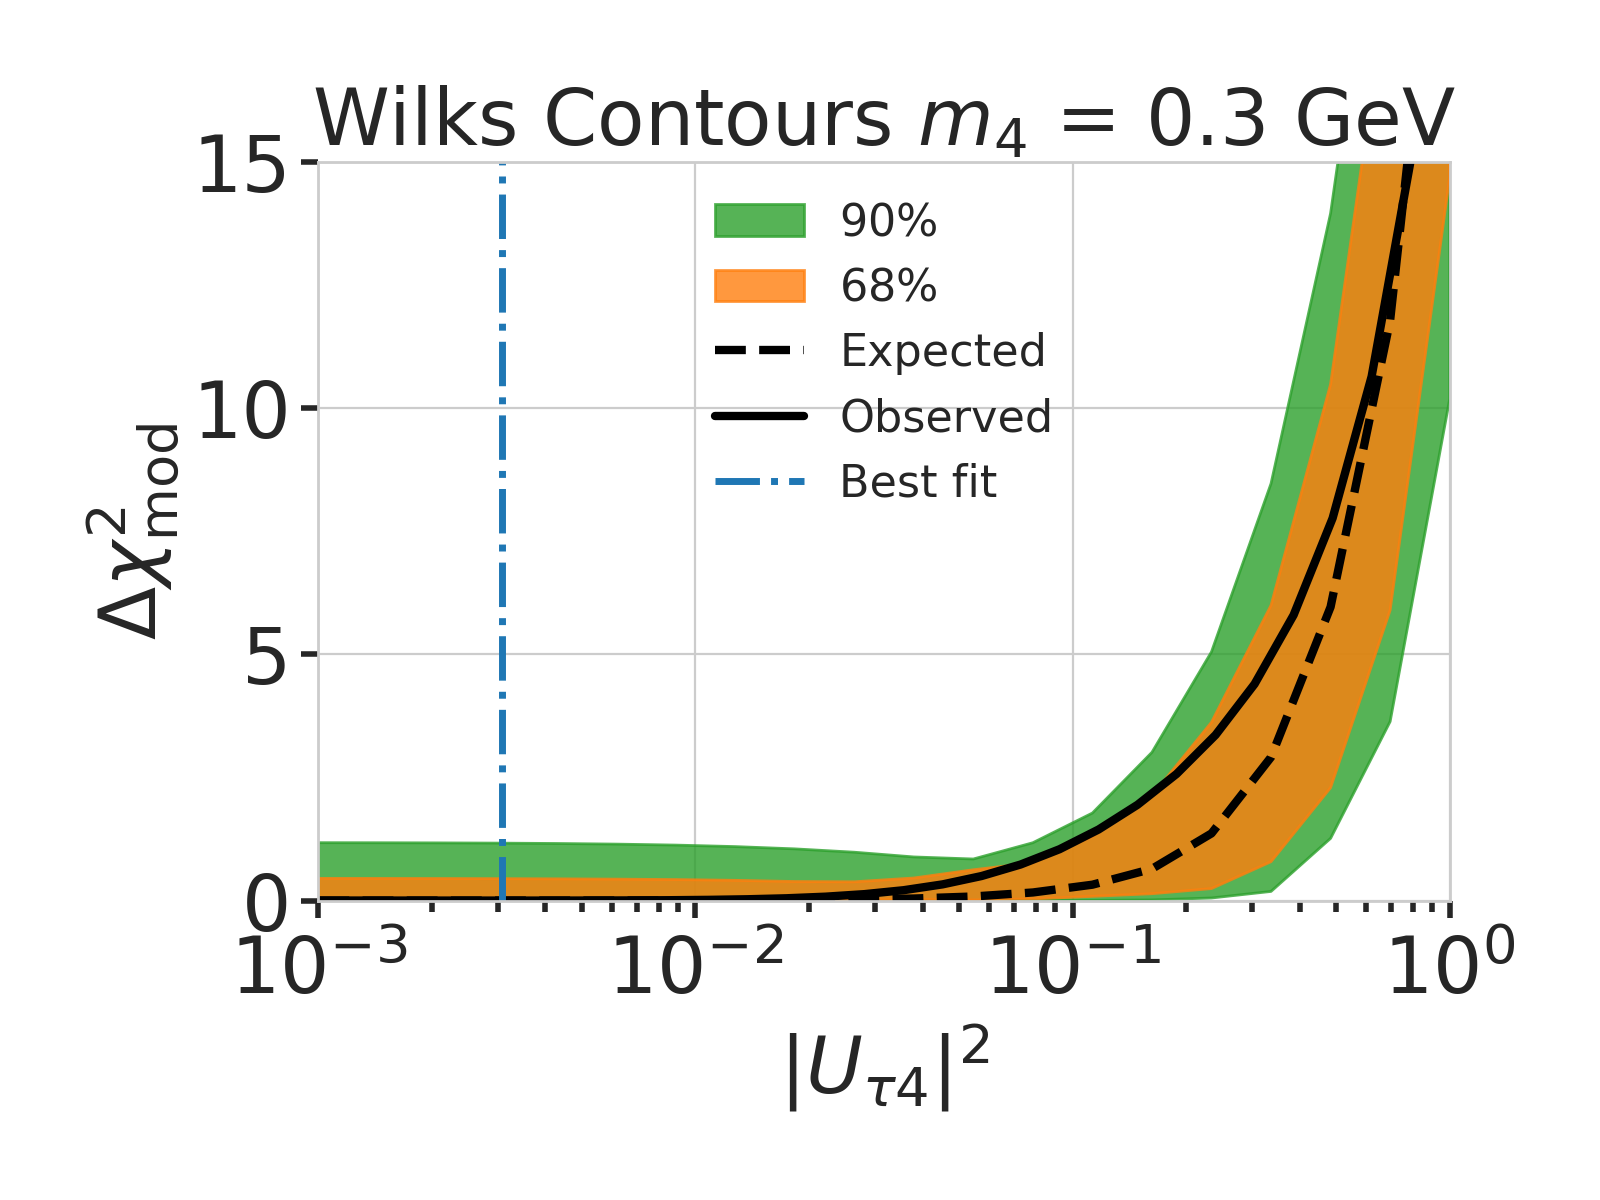
\includegraphics[width=0.32\linewidth]{figures/results/best_fit/brazil_band_with_asimov_0.3_GeV_with_bfp.png}
    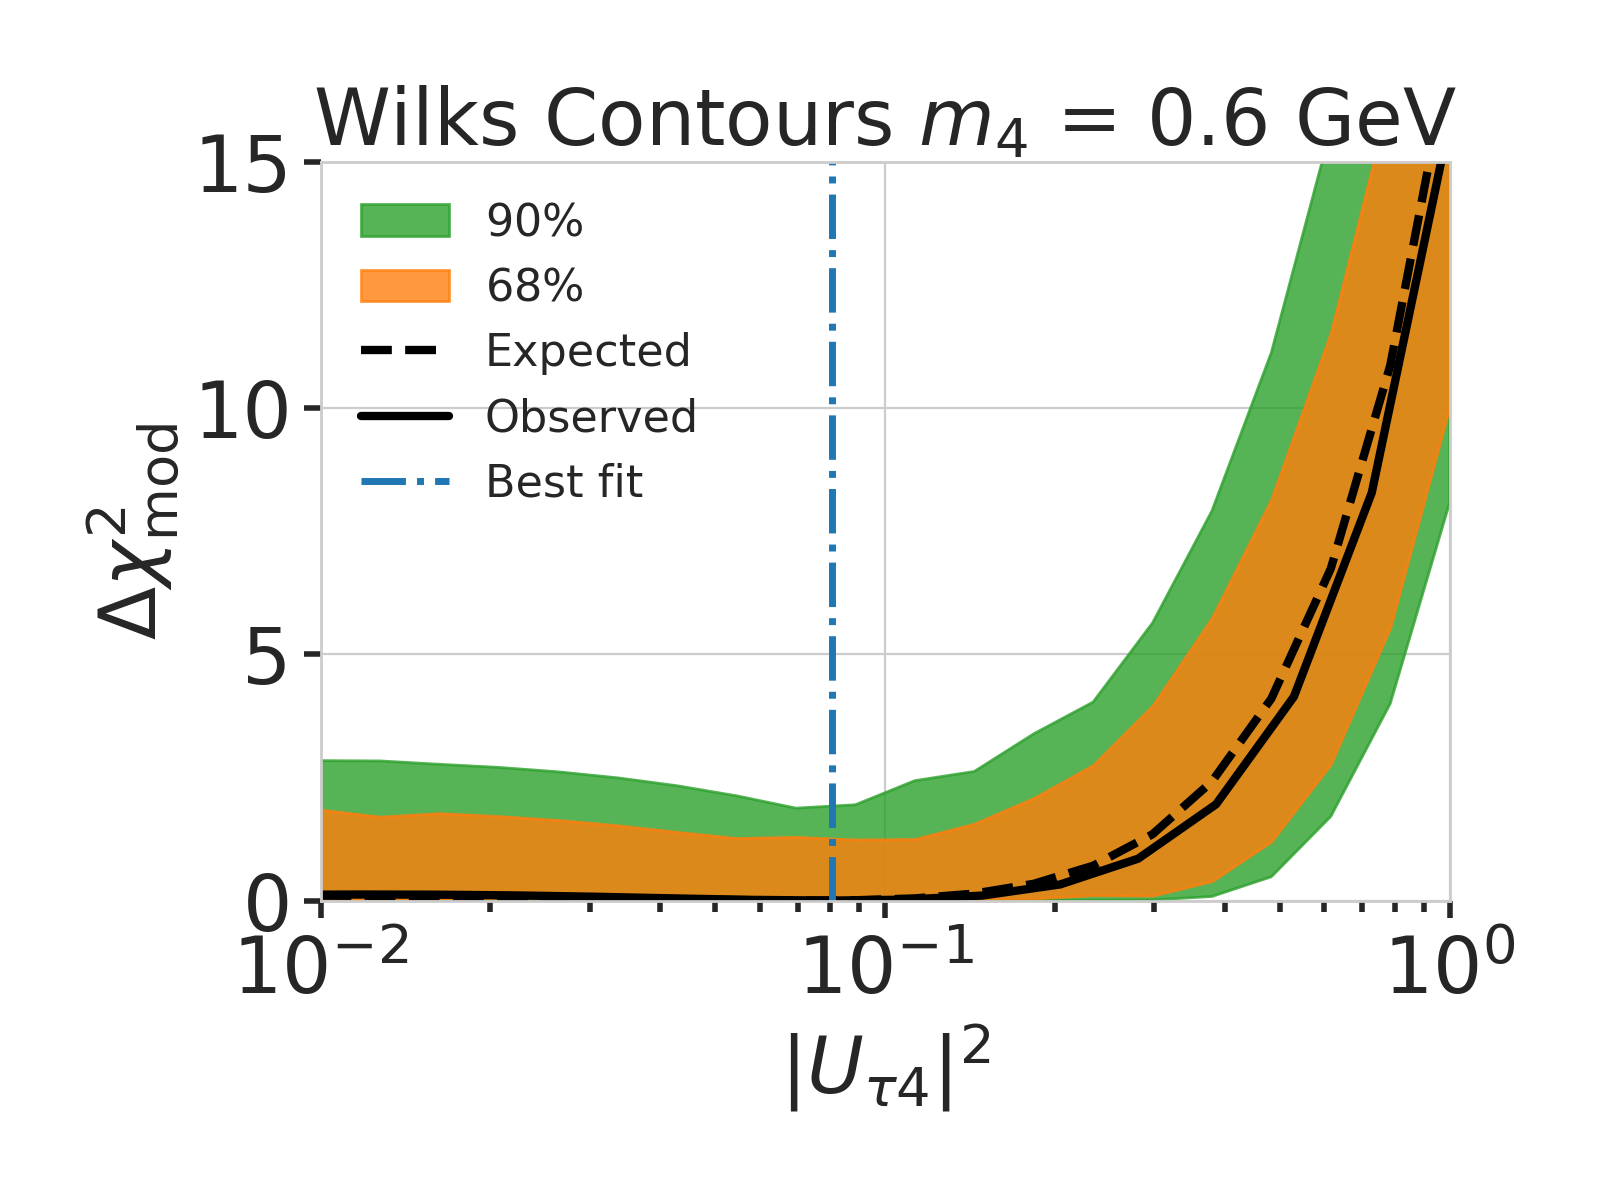
\includegraphics[width=0.32\linewidth]{figures/results/best_fit/brazil_band_with_asimov_0.6_GeV_with_bfp.png}
    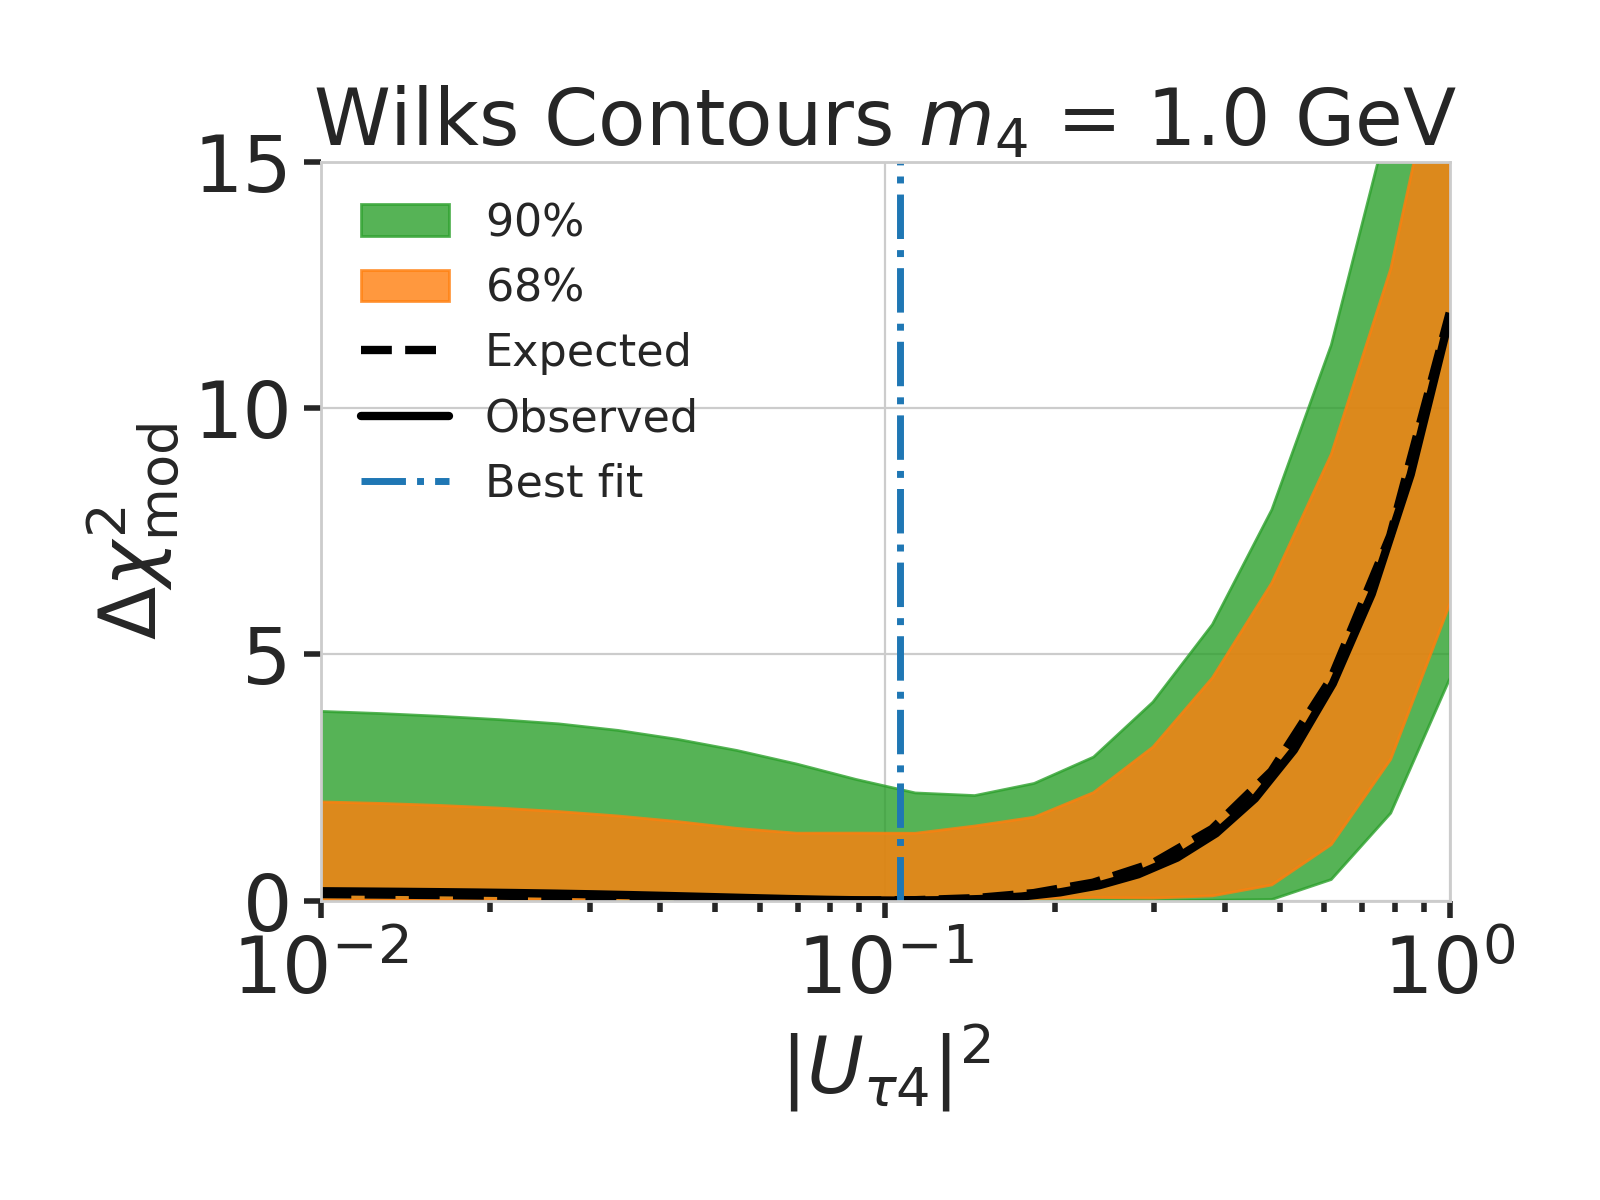
\includegraphics[width=0.32\linewidth]{figures/results/best_fit/brazil_band_with_asimov_1.0_GeV_with_bfp.png}
	\caption[xx]{xx}
    \labfig{brazil_bands}
\end{figure*}
\todo{fix caption for this figure (RED)}


% \begin{figure}[h]
%     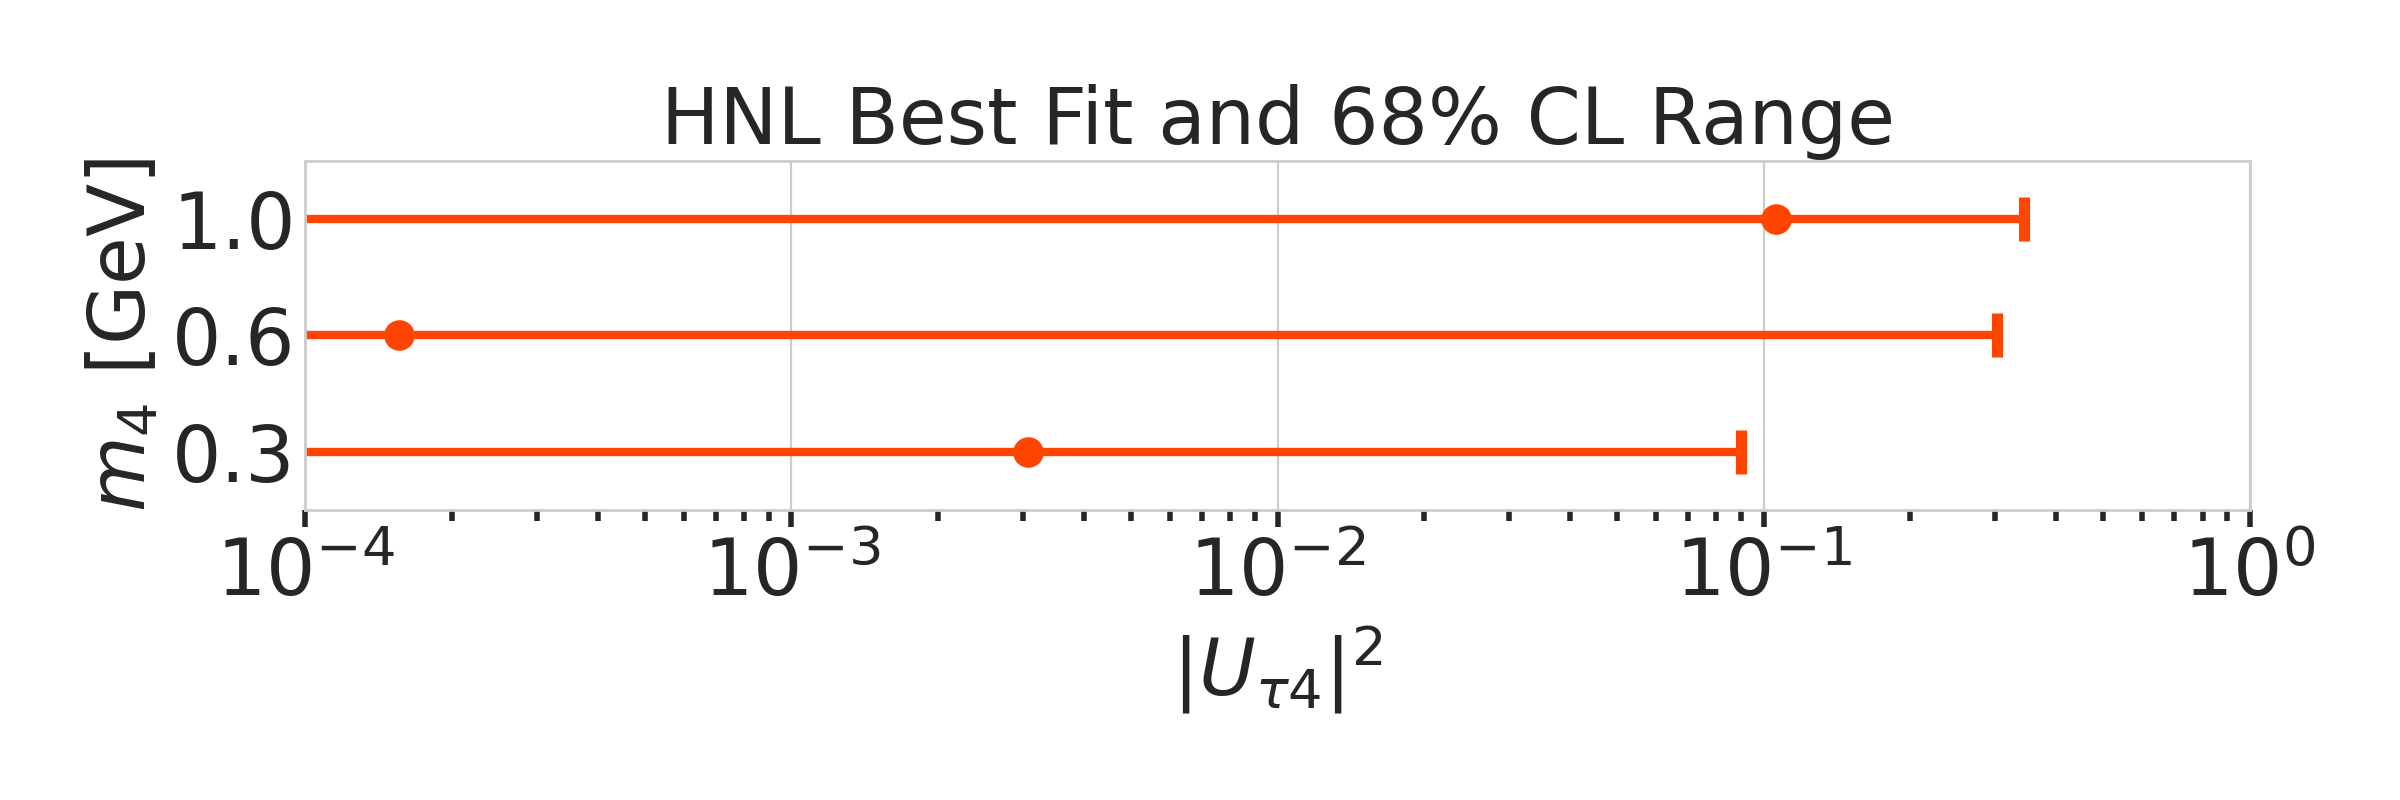
\includegraphics{figures/results/best_fit/best_fit_results_and_limits.png}
% 	\caption[xx]{xx}
%     \labfig{best_fit_mixings_and_limit}
% \end{figure}
% \todo{fix caption for this figure}

\todo{make plot with BFPs and limit, comparing to upper limits from other experiments, think about how to present it (RED)}


% \subsection{Likelihood Coverage}

% To find the CLs, the profile likelihood was evaluated by applying Wilks' theorem. It is not guaranteed however, that the theorem holds, and it is therefore important to check the \textit{coverage} of the likelihood. For a chosen CL, like the \SI{90}{\percent} CL, the coverage is tested by calculation the fraction of measurements with pseudo-data that fall within this region. The likelihood is said to be \textit{under-covering}, if fewer than \SI{90}{\percent} of the pseudo-data trials fall within the \SI{90}{\percent} CL contour. Oppositely, \textit{over-covering} means that more than \SI{90}{\percent} of the pseudo-data trials fall within the same contour. The coverage depends on the assumed true parameter values, and it is therefore checked at particular values that are interesting. For this analysis, the coverage is checked at several values of $|U_{\tau4}|^2$ between the BFP and the position of the \SI{90}{\percent} CL limit\todo{Does that make sense, do I need less, or even more? One mass sample, or all?}. Pseudo-data is generated at these points and two fits are run, one where the mixing is free and one where it is fixed to the true values. The coverage is assessed by counting the fraction of trials where the $\Delta\chi^2_{\mathrm{mod}}$ between the two fits is smaller than the threshold provided by Wilks' theorem. \reffig{coverage_0.6_GeV} shows the coverage for the \SI{0.6}{\gev} mass sample, where the coverage is found to be slightly under-covering/over-covering\todo{fix this with the real result}. The same is true for the other two mass samples and the corresponding plots can be found in \refsec{coverage_appendix}. This means that the CLs shown in \reftab{best_fit_parameters_and_confidence_levels} are slightly conservative/optimistic.

